%\setchapterpreamble[u]{\margintoc}
\chapter{Complex calculus}
\label{h:complex}

\begin{quote}
The shortest path between two truths in the real domain passes through the complex domain.

--- Jacques Hadamard
\end{quote}

\begin{quote}
The imaginary number is a fine and wonderful recourse of the divine spirit, almost an amphibian between being and not being.

--- Gottfried Wilhelm Leibniz
\end{quote}

\begin{quote}
  Life is complex: it has both real and imaginary components.
  
--- Rich Rosen
\end{quote}

In this chapter, we will discuss the basic principles of complex analysis and its applications.

We will define functions of a complex variable and show how to differentiate and integrate them. In order to facilitate the calculation of integrals, residue calculus is introduced. This will give us a powerful tool to also calculate some real-valued integrals in a much more straightforward way. Finally, we discuss conformal transformations as a way to map problems to equivalent ones having an 'easier' geometry. 

We will also study a number of direct applications of complex analysis, e.g. the Kramers--Kronig dispersion relations, and the use of conformal transformations to model waveguide bends.

\chaptertoc{}

\pagebreak


\sectionugent{Functions of a complex variable}

A function of a complex variable is simply defined as

\begin{equation}
f(z) \stackrel{def}{=} f(x + j y) \stackrel{def}{=}  u(x,y) + j v(x,y)
\end{equation}

Here, $u$ and $v$ are two real--valued functions of $x$ and $y$. Unsurprisingly, we call $u$ the real part of $f$ and $v$ the imaginary part of $f$.

\begin{cue}
Take
$$u = x^2 - y^2$$
$$v = 2 x y$$
What is $f(z)$?
\end{cue}

In this case,

$$f(z) = u + j v = x^2 - y^2 +2j x y = (x + jy)^2$$

So, formally we can say that $u$ and $v$ define the function $f(z) = z^2$

\begin{cue}
Given
$$f(z) = z z^* $$
such that
$$f(z) = (x + jy)(x - jy) = x^2 + y^2$$

What are the corresponding $u$ and $v$?
\end{cue}

The real and imaginary parts are:

$$u = x^2 + y^2$$
$$v = 0$$


\pagebreak


\sectionugent{Derivatives of complex functions}

Let us now differentiate complex functions. In analogy with real--valued functions, we would like to define the complex derivative as

\begin{equation}
f' (z)=\frac{df}{dz} \stackrel{def}{=} \lim_{\Delta z \to 0} \frac{f(z+\Delta z) - f(z)}{z+\Delta z - z} \label{eq-deriv}
\end{equation} 

\begin{cue}
Use this definition to find the derivative of $f(z)=z^2$.
\end{cue}

To calculate the derivative of  $f(z)=z^2$, we find that

$$f'(z)=\lim_{\Delta z \to 0} \frac{(z+\Delta z)^2 - z^2}{\Delta z} = \lim_{\Delta z \to 0} \frac{2 z \Delta z - (\Delta z)^2}{\Delta z}=2z $$

This gives the same result as in the real-valued case.

At this point, you might wonder what all the fuzz is about, as complex analysis seems to boil down to simply replacing $x$ by $z$. However, there's more going on than meets the eye.

\begin{cue}
Try to find the derivative of $f(z)=|z|^2$.
\end{cue}

In this case, we get

$$f'(z)=\lim_{\Delta z \to 0} \frac{|z+\Delta z|^2 - |z|^2}{\Delta z} $$

The numerator is obviously real-valued, but the denominator is in general complex, so that the result of this operation would depend on the direction of approach encoded in $\Delta z$.

This is obviously undesirable. Now, we can ask ourself the question, what are the conditions under which the derivative Eq.~\ref{eq-deriv} of a complex function is independent of the direction of approach?

\begin{marginfigure}[-2cm]
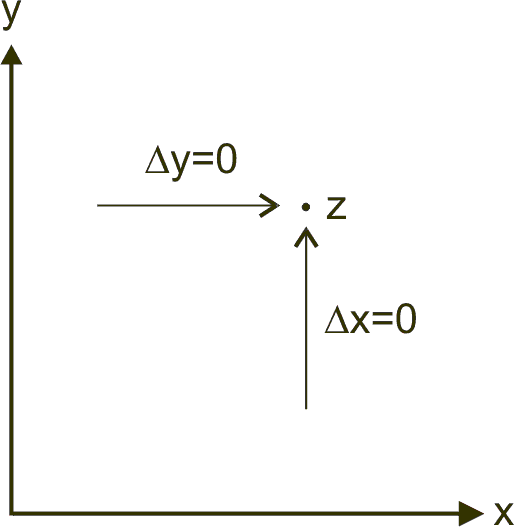
\includegraphics[width=4cm]{complex/figures/approach_z}
\caption{Different approaches to $z$ in the complex plane.}
\label{fig-approach-z}
\end{marginfigure}

Let's have a look at the necessary conditions first. If the direction of approach does not matter at all, than we should certainly get the same result if we pick two special directions (see Fig.~\ref{fig-approach-z}).

\begin{cue}
 By splitting both $f$ and $z$ into their real and imaginary components, take the limit of $\Delta f / \Delta z$ along the horizontal direction.
\end{cue}

Along the horizontal direction, $\Delta y = 0$, so taking the limit $\Delta x \to 0$, we get

\begin{align}
\lim_{\Delta z \to 0} \frac{\Delta f}{\Delta z}
& = \lim_{\Delta z \to 0} \frac{\Delta u + j \Delta v}{\Delta x + j \Delta y}
\nonumber \\
& = \lim_{\Delta x \to 0} \frac{\Delta u}{\Delta x} + j \frac{\Delta v}{\Delta
x} \nonumber \\
& = \frac{\partial u}{\partial x} + j \frac{\partial v}{\partial
x}\label{eq-deriv-dx}
\end{align} 

\begin{cue}
Do the same for an approach along the vertical direction.
\end{cue}

Along the vertical direction, $\Delta x = 0$ and we should take the limit $\Delta y \to 0$:

\begin{align}
\lim_{\Delta z \to 0} \frac{\Delta f}{\Delta z}
& = \lim_{\Delta z \to 0} \frac{\Delta u + j \Delta v}{\Delta x + j \Delta y}
\nonumber \\
& = \lim_{\Delta y \to 0} -j\frac{\Delta u}{\Delta y} +  \frac{\Delta v}{\Delta
y} \nonumber \\
& = -j\frac{\partial u}{\partial y} +  \frac{\partial v}{\partial
y}\label{eq-deriv-dy}
\end{align}

\begin{cue}
Now derive a necessary condition for the complex derivative to be independent of the direction of approach.
\end{cue}

A necessary condition for the complex derivative to be independent of the direction of approach, can be derived from equating the real and imaginary parts of Eq.~\ref{eq-deriv-dx} and \ref{eq-deriv-dy}:

\begin{equation}
\fbox{$\displaystyle
\frac{\partial u}{\partial x} = \frac{\partial v}{\partial y}, \hspace{.5cm}
\frac{\partial v}{\partial x} = -\frac{\partial u}{\partial y}
\label{eq-Cauchy-Riemann}
$}
\end{equation} 

\begin{marginfigure}[-4.0cm]
  % credits: Wikipedia
  % url: https://en.wikipedia.org/wiki/Bernhard_Riemann#/media/File:Georg_Friedrich_Bernhard_Riemann.jpeg
  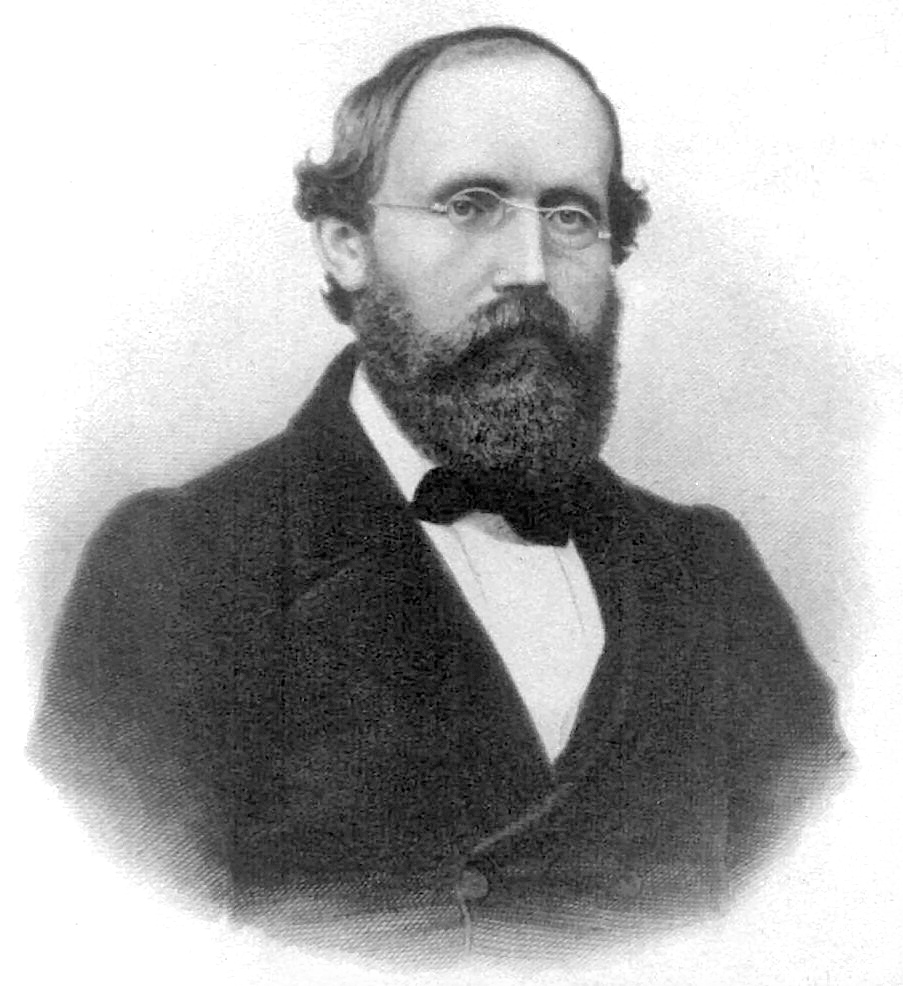
\includegraphics{complex/figures/b_riemann}
  \caption{Bernhard Riemann (1826-1866)}
\end{marginfigure}

These are called the \emph{Cauchy--Riemann conditions}. A complex function that satisfies these conditions is called \emph{analytic} (or holomorphic). Important to note is that for a function to be analytic, it necessarily has to be continuous and should not contain any singularities, otherwise the derivative would certainly be undefined.

We will now show that the Cauchy--Riemann conditions are not only necessary, they are also sufficient (assuming all partial derivatives are continuous).

We can write the total differential

\begin{equation}
d f = \left( \frac{\partial u}{\partial x}+j\frac{\partial v}{\partial x}\right) d x+\left(\frac{\partial u}{\partial y}+j\frac{\partial v}{\partial y}\right) d y
\end{equation} 

such that

\begin{equation}
\frac{d f}{d z} = \frac{\left(\frac{\partial u}{\partial x}+j\frac{\partial v}{\partial x}\right) d x+\left(\frac{\partial u}{\partial y}+j\frac{\partial v}{\partial y}\right) d y}{d x + j d y}
\end{equation} 

or

\begin{equation}
\frac{d f}{d z} = \frac{\left(\frac{\partial u}{\partial x}+j\frac{\partial v}{\partial x}\right) +\left(\frac{\partial u}{\partial y}+j\frac{\partial v}{\partial y}\right) \frac{d y}{d x}}{1 + j \frac{d y}{d x}} \label{eq-cr-suf}
\end{equation} 

\begin{cue}
Where in Eq.~\ref{eq-cr-suf} is the direction of approach encoded? Get rid of that term by applying the Cauchy-Riemann conditions.
\end{cue}

We now need to prove that this expression is independent on $d y / d x$ in order for the complex derivatives to be independent of the direction of approach. Indeed, each direction of approach will have its own value of $d y / d x$ .

Applying the Cauchy--Riemann conditions to the $y$--derivatives, we obtain

\begin{equation}
\frac{\partial u}{\partial y}+j\frac{\partial v}{\partial y} = -\frac{\partial v}{\partial x}+j\frac{\partial u}{\partial x}
\end{equation}

Substituting this into Eq.\ref{eq-cr-suf}, we get that the $d y / d x$ dependence cancels out to give

\begin{equation}
\fbox{$\displaystyle
\frac{d f}{d z} = \frac{\partial u}{\partial x}+j\frac{\partial v}{\partial x}
$}
\end{equation} 

This equation also shows that only derivatives with respect to $x$ are needed to calculate the complex derivative.

\pagebreak

\begin{exer}
% difficulty: trivial
% ugent
Are the following functions analytic? If so, calculate their derivative.
$$\begin{array}{lcll}a) & f(z)=z^2 \\b) & f(z)=z z^* \\c) & f(z)= \Re(z)=x \end{array}$$

What rule-of-thumb can you derive from these results?

\begin{sol}
Analytical and $f'(z)=2z$ / non-analytical / non-analytical. Real-valued functions where you replace $x$ by $z$ are typically analytical. Functions where you make explicit reference to the real and imaginary components of a complex number or to its complex conjugate are not.
\end{sol}
  
\end{exer}

\begin{exer}
% difficulty: normal
\label{ex-harmonic}
$u$ and $v$ are the real and imaginary parts, respectively, of an analytic function $f(z)$. Show that $u$ and $v$ are \emph{harmonic} functions, i.e. they satisfy Laplace's equation
$$\nabla^2 u = \nabla^2 v = 0$$
\end{exer}

\begin{exer}
 % difficulty: normal
$u$ and $v$ are the real and imaginary parts, respectively, of an analytic function $f(z)$. Show that $|f'(z)|^2$ is equal to the Jacobian determinant
$$\frac{\partial (u,v)}{\partial (x,y)} =  \begin{vmatrix} \partial u / \partial x & \partial u / \partial y \\ \partial v / \partial x & \partial v / \partial y \end{vmatrix}$$
\end{exer}


\pagebreak


\sectionugent{Integrals of complex functions}

With differentiation under control, it is time to study integrals of complex functions. The integral of a complex function along a specified path ${C}$ between $z_0$ and $z_1$ (see Fig.~\ref{fig-integral}) is defined by

\begin{marginfigure}[]
\centering
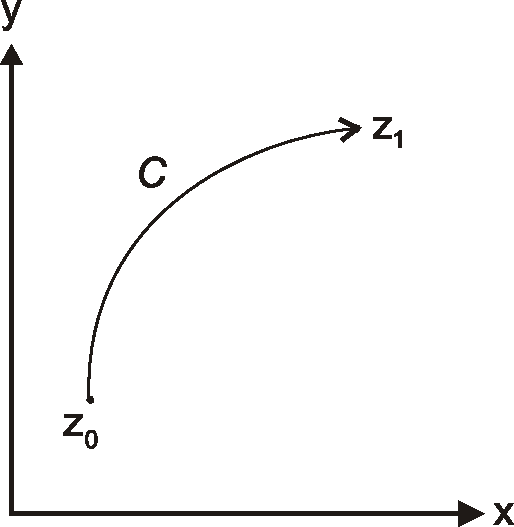
\includegraphics{complex/figures/integral}
\caption{A complex line integral.}
\label{fig-integral}
\end{marginfigure}

\begin{align}
\int_{C}f(z)dz = & \int_{C}\left(u(x,y)+jv(x,y)\right)(dx+jdy)
\nonumber \\
  = & \int_{C}\left[u(x,y)dx-v(x,y)dy\right] + \nonumber\\
  & j\int_{C}\left[v(x,y)dx+u(x,y)dy\right] \label{eq-complex-int}
\end{align} 

So, the integral of a complex function has been expressed in terms of well-known real line integrals, which are calculated in the normal way by parametrisation of the curve. (Note that in Eq.~\ref{eq-complex-int} $dx$ and $dy$ are not independent, but related by the choice of the integration path.)

Let's calculate the contour integral $\oint_{C}z^ndz$ where the contour ${C}$ is a counterclockwise circular path of radius $r$ around the origin $z=0$. Note that we do not necessarily need to split up the integral into its real and imaginary components, but that we can directly parametrise the complex path if we want.

\begin{cue}
Parametrise the curve in polar coordinates using $z=r\exp(j\theta)$ for $\theta=0\to 2 \pi$ and calculate the integral. 
\end{cue}

Expressing the unit cirle as $z=r\exp(j\theta)$ for $\theta=0\to 2 \pi$, we get

$$\oint_{C} z^n dz = \int_0^{2\pi} \left(r^n e^{jn\theta}\right) \left(jr e^{j \theta}d \theta\right)=j r^{n+1} \int_0^{2\pi} e^{j(n+1)\theta} d \theta $$

For $n \neq -1$ this is equal to

$$ \frac{r^{n+1}}{n+1}\left[e^{j(n+1)\theta}\right]_0^{2\pi}=0 $$

because of the periodicity of the exponential. For $n=-1$, we obtain 

$$ \oint_{C} \frac{dz}{z} = j \int_0^{2\pi} d \theta = 2 \pi j $$

which is independent of $r$.

Note that the results of this seemingly trivial integral will prove to have deep consequences later.

\begin{exer}
% difficulty: trivial
Use parametrisation to calculate the integral

$$\int_{z_0}^{z_1} dz$$

for any given points $z_0$ and $z_1$.
\end{exer}


\pagebreak


\sectionugent{Cauchy's integral theorem}

\begin{marginfigure}[+0.3cm]
  % credits: Wikipedia
  % url: https://en.wikipedia.org/wiki/Augustin-Louis_Cauchy
  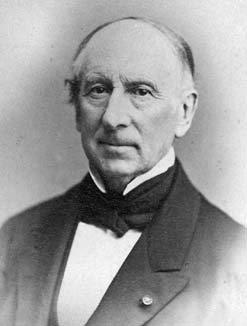
\includegraphics{complex/figures/cauchy}
  \caption{Augustin-Louis Cauchy (1789-1857)}
\end{marginfigure}

One of major theorems in complex calculus is Cauchy's integral theorem. It states that 

\begin{equation}
\fbox{$\displaystyle
\oint_{{C}} f(z) dz = 0 \label{eq-cauchy-1}
$}
\end{equation}

Important to note is that Eq.~\ref{eq-cauchy-1} only holds if $f(z)$ is analytic for all the points enclosed by the contour ${C}$, as well as for the points on the contour itself. The symbol $\oint$ is used to emphasise that the path is closed.

\begin{cue}
To prove Eq.~\ref{eq-cauchy-1}, first apply the definition of the complex contour integral given in Eq.~\ref{eq-complex-int}.
\end{cue}

This gives

\begin{align}
\oint_{C}f(z)dz = & \oint_{C}\left(u(x,y)+jv(x,y)\right)(dx+jdy)
\nonumber \\
  = & \oint_{C}\left[u(x,y)dx-v(x,y)dy\right] + \nonumber \\
  & j \oint_{C}\left[v(x,y)dx+u(x,y)dy\right]  \label{eq-cauchy-proof}
\end{align}

\begin{marginfigure}[-0.0cm]
  % credits: Wikipedia
  % url: https://en.wikipedia.org/wiki/Sir_George_Stokes,_1st_Baronet#/media/File:Ggstokes.jpg
  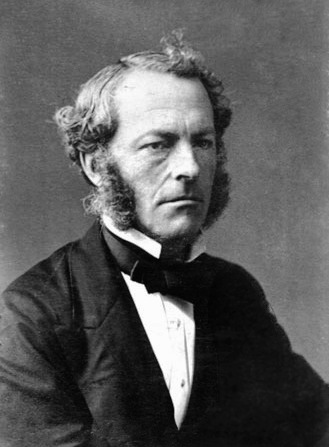
\includegraphics{complex/figures/stokes}
  \caption{George Stokes (1819-1903)}
\end{marginfigure}

In order to be able to use the Cauchy-Riemann conditions, we somehow need to bring partial derivatives into this formula. For this, we will use Stokes's theorem:

\begin{equation}
\oint_{{{C}}} {\mathbf A} \cdot d {\mathbf l} = \iint_S \nabla \times {\mathbf A} \cdot d {\mathbf S}
\end{equation}

\begin{cue}
Convert Stokes's theorem to our two-dimensional case.
\end{cue}

In two dimensions (i.e. $A_z=0$ and the contour contained in the $(x,y)$--plane), Stokes becomes:

\begin{equation}
\oint_{{C}} \left(A_x dx + A_y dy\right) = \iint_S \left(\frac{\partial
A_y}{\partial x} - \frac{\partial A_x}{\partial y} \right)dx dy
\end{equation} 

\pagebreak

\begin{cue}
Figure out which values of $A_x$ and $A_y$ to use, so that we can apply Cauchy--Riemann to the first term in Eq.~\ref{eq-cauchy-proof}.
\end{cue}

For the first term in Eq.~\ref{eq-cauchy-proof}, we choose $A_x=u$ and $A_y=-v$ such that

\begin{align}
\oint_{C}\left[u(x,y)dx-v(x,y)dy\right] =& \oint_{{C}} \left(A_x dx + A_y dy\right) \nonumber \\
=& \iint_S \left(\frac{\partial A_y}{\partial x} - \frac{\partial A_x}{\partial y} \right)dx dy \nonumber \\ =& -\iint_S \left(\frac{\partial v}{\partial x} + \frac{\partial u}{\partial y} \right)dx dy 
\end{align} 

Because of the Cauchy--Riemann conditions Eq.~\ref{eq-Cauchy-Riemann}, this
vanishes.

\begin{cue}
Which values of $A_x$ and $A_y$ should we use for the second term in Eq.~\ref{eq-cauchy-proof}?
\end{cue}

A similar conclusion can be drawn for the second term in Eq.~\ref{eq-cauchy-proof} by setting $A_x=v$ and $A_y=u$, which proves that the entire integral in Eq.~\ref{eq-cauchy-1} vanishes.

\begin{exer}
% difficulty: trivial
Prove that for an analytic function $f(z)$ the line integral 
$$\int_{z_0}^{z_1}f(z)dz$$
is independent on the exact path between $z_0$ and $z_1$.
\end{exer}


\pagebreak


\sectionugent{Cauchy's integral formula}

The second major theorem in complex calculus is Cauchy's integral \emph{formula} (as opposed to Cauchy's integral \emph{theorem} from the previous section). Cauchy integral formula states that for an analytic function $f(z)$

\begin{equation}
\fbox{$\displaystyle
\frac{1}{2 \pi j}\oint_{{C}} \frac{f(z)} {z-z_0} dz = f(z_0)
\label{eq-cauchy-2}
$}
\end{equation}

Important here is that $z_0$ is a point enclosed by the contour ${C}$.

\begin{cue}
What would happen to Eq.~\ref{eq-cauchy-2} if  $z_0$ were outside of the contour?  
\end{cue}

If $z_0$ were outside of the contour, then the integrand of Eq.~\ref{eq-cauchy-2} would be analytic in the entire region enclosed by the contour. In that case, Cauchy's theorem applies and the integral vanishes.

\begin{marginfigure}[-1cm]
\centering
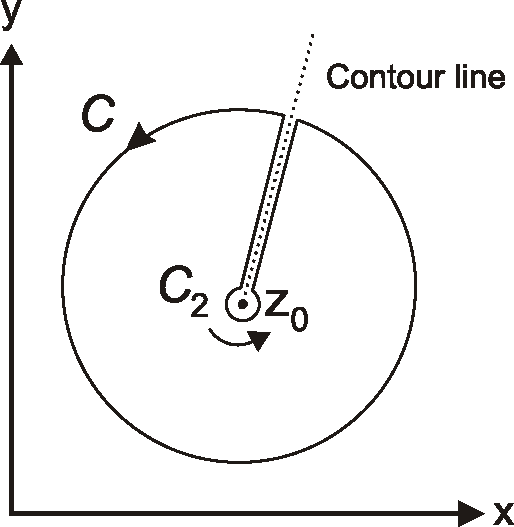
\includegraphics[width=5cm]{complex/figures/cauchy_II}
\caption{Contour to prove Cauchy's formula.}
\label{fig-cauchy-II}
\end{marginfigure}

To prove Eq.~\ref{eq-cauchy-2}, we note that although the function $f(z)$ is analytic, $f(z)/(z-z_0)$ is not, because is has a singularity at $z=z_0$. However, if we deform ${C}$ to exclude the singularity as in Fig.~\ref{fig-cauchy-II}, we end up with a contour where Cauchy's theorem does apply.

\begin{cue}
Apply Cauchy's theorem to this extended contour, splitting up the contributions from its different parts.
\end{cue}

The result is

\begin{equation}
\oint_{{C}} \frac{f(z)} {z-z_0} dz -\oint_{{C}_2} \frac{f(z)}
{z-z_0} dz=0
\end{equation} 

Here, ${C}$ is the original outer contour and ${C}_2$ is the circle surrounding the point $z_0$ traversed in a counterclockwise direction (hence the minus sign). The two sections of the path along the contour line cancel because $f(z)$ is continuous (a side effect of it being analytic).

\begin{cue}
Parametrise ${C}_2$ and calculate its contribution to the integral. Then, take the limit $ r \to 0 $ to prove Cauchy's formula.   
\end{cue}

To calculate the integral along ${C}_2$, we use the parametrisation $z=z_0 + r e^{j\theta}$:

\begin{equation}
\oint_{{C}_2} \frac{f(z)} {z-z_0} dz = \oint_{{C}_2} \frac{f(z_0
+ r e^{j\theta})} {r e^{j\theta}} \left(rje^{j \theta} d \theta\right)
\end{equation}

In the limit $ r \to 0 $ this becomes

\begin{align}
\oint_{{C}_2} \frac{f(z)} {z-z_0} dz = & \, j f(z_0) \oint_{{C}_2} d \theta \nonumber \\
 = & \, 2 \pi j f(z_0)
\end{align}
 
which proves Cauchy's integral formula.

Note that this formula is quite remarkable. It means that as soon as the values of an analytic function are specified on a contour, we immediately know the function values at all the interior points.

\begin{exer}
% difficulty: trivial
% ugent
Use Cauchy's formula to calculate 
$$\oint_{{C}}  \frac {e^z} {z+1} dz$$
Here ${C}$ is a circle of radius 4 centered at the origin.
\begin{sol}
$$\frac{2 \pi j}{e}$$
\end{sol}
\end{exer}

\begin{exer}
% difficulty: normal
Use Cauchy's formula to calculate 
$$\oint_{{C}}  \frac {e^{az}} {z} dz$$
Here ${C}$ is the unit circle and $a$ is a real-valued constant. Then, write this integral in terms of $\theta$ and show
$$ \int_0^\pi e ^{a \cos \theta} \cos (a \sin \theta) d\theta = \pi $$
\begin{sol}
$$2 \pi j$$
\end{sol}
\end{exer}

\begin{exer}
% difficulty: hard
% ugent
\label{ex-cauchy-diff}
Prove the following identity:

$$f'(z_0)=\frac{1}{2 \pi j} \oint_{{C}} \frac{f(z)} {(z-z_0)^2} dz$$

This expression can be used to (numerically) calculate the derivative of an analytic function.
\begin{hnt}
Apply Cauchy's formula to each of the terms of $$\frac{f(z_0+\Delta z_0) - f(z_0)}{\Delta z_0}$$ Then take the limit ${\Delta z_0} \to 0$.
\end{hnt}
\end{exer}

\begin{exer}
% difficulty: hard
Show that

  $$f^{(n)}(z_0)=\frac{n!}{2 \pi j} \oint_{{C}} \frac{f(z)} {(z-z_0)^{n+1}} dz$$
  
This also means that if a function is analytic, then the derivatives of any order automatically exist.
\begin{hnt}
Repeating the technique used in Ex. \ref{ex-cauchy-diff}.
\end{hnt}  
\end{exer}


\pagebreak


\sectionugent{Laurent series}


\begin{marginfigure}
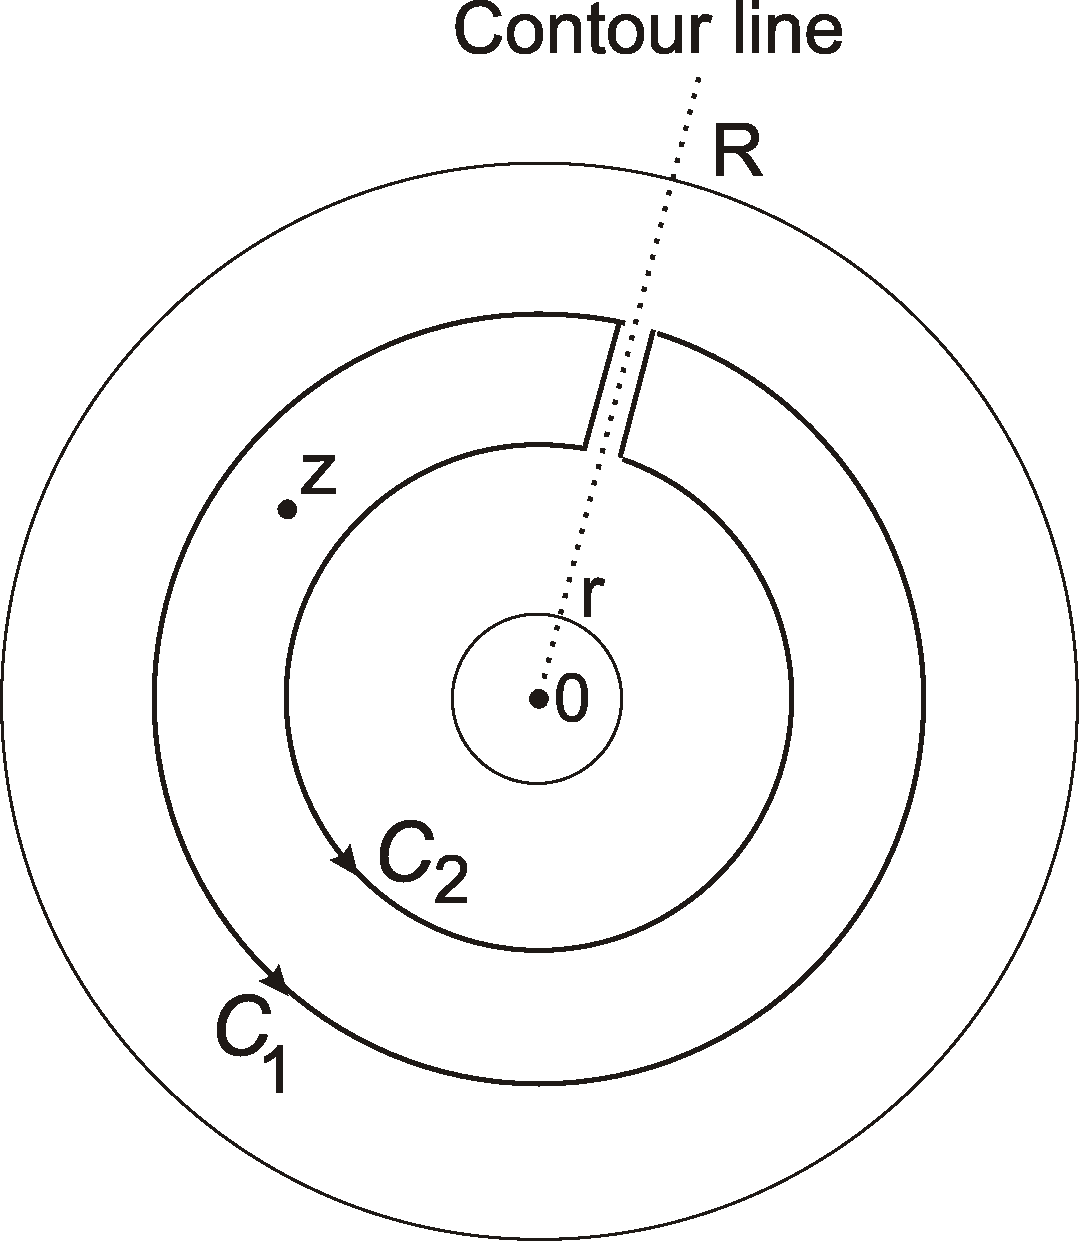
\includegraphics{complex/figures/laurent}
\caption{Contour to derive Laurent series.}
\label{fig-laurent}
\end{marginfigure}

Let's try to come up with a series expansion for complex functions. Here, special care has to be taken with respect to the convergence area. Consider e.g. a function that is analytic in some annular region around the origin of inner radius $r$ and outer radius $R$. A simple circular contour would enclose the inner region where the function is not analytic, so we need to construct a more complicated contour that only encloses points where the function is analytic (Fig.~\ref{fig-laurent})

\begin{cue}
  Apply Cauchy's formula, splitting up the contour into its different parts.
\end{cue}

Cauchy's formula gives us

\begin{equation}
f(z)=\frac{1}{2 \pi j }\oint_{{C}_1} \frac{f(z')} {z'-z} dz' -\frac{1}{2
\pi j }\oint_{{C}_2} \frac{f(z')} {z'-z} dz' \label{laurent_0}
\end{equation} 

Here, $z$ is a fixed point on the inside of the contour, while $z'$ is the integration variable running along the contour. The two line segments cancel once again.

Our aim is to transform this formula into a series expansion. One can prove that the following straightforward generalisation of the well--known geometric series expansion holds:

\begin{equation}
\frac{1}{1-z} = \sum_{n=0}^\infty z^n, \hspace{.5cm} |z| < 1
\end{equation}

\begin{cue}
Manipulate the different terms in Eq.~\ref{laurent_0} so that we are able to use the geometric series. Pay special attention to the radius of convergenc, by dividing the numerator and denominator by $z$ or $z'$.
\end{cue}

Simple manipulation of Eq.~\ref{laurent_0} yields

\begin{equation}
f(z)=\frac{1}{2 \pi j }\oint_{{C}_1} f(z') \frac{1 / z'} {1-z / z'} dz' + \frac{1}{2 \pi j }\oint_{{C}_2} f(z') \frac{1 / z} {1 - z' / z} dz'
\label{eq-laurent-1}
\end{equation} 

Note that $z$ is on the inside of ${C}_1$, such that $| z | < |z'| $, or $ |z / z' | < 1$ in the first term in Eq.~\ref{eq-laurent-1}. Similarly, $z$ is on the outside of ${C}_2$, such that $|z'| < | z | $, or $ |z'  / z| <
1$ in the second term in Eq.~\ref{eq-laurent-1}.

With this, we can write Eq.~\ref{eq-laurent-1} as

\begin{equation}
f(z)=\frac{1}{2 \pi j }\oint_{{C}_1} \frac{f(z')}{z'} \sum_{m=0}^{\infty} \left( \frac{z}{z'}\right)^m dz' + \frac{1}{2 \pi j }\oint_{{C}_2} \frac{f(z')}{z} \sum_{n=0}^{\infty} \left(\frac{z'}{z}\right)^n dz'
\end{equation}

\begin{cue}
Clean up this formula so that the coefficients of the power series become clearly visible.
\end{cue}

Provided we can exchange summation and integration, we can write

\begin{equation}
f(z)=\frac{1}{2 \pi j } \sum_{m=0}^{\infty} z^m \oint_{{C}_1} \frac{f(z')}{z^{\prime (m+1)}} dz' + \frac{1}{2 \pi j } \sum_{n=0}^{\infty} z ^ {-n-1} \oint_{{C}_2}  {f(z')}  (z')^ n dz'
\end{equation} 

or more symmetrically

\begin{equation}
f(z)=\frac{1}{2 \pi j } \sum_{m=0}^{\infty} z^m \oint_{{C}_1} \frac{f(z')}{z^{\prime (m+1)}} dz' + \frac{1}{2 \pi j } \sum_{n=1}^{\infty} z ^ {-n} \oint_{{C}_2} \frac{f(z')}{z^{\prime^ {(-n+1)}}} dz'
\label{eq-laurent-int}
\end{equation} 

This means that we can expand $f(z)$ in a power series containing both negative and positive powers of $z$:

\begin{equation}
f(z)= \sum_{m=-\infty}^{\infty} a_m z^m
\end{equation} 

\begin{marginfigure}[-.0cm]
  % credits: Wikipedia
  % url: https://upload.wikimedia.org/wikipedia/commons/d/d8/Pierre_Alphonse_Laurent.jpeg
  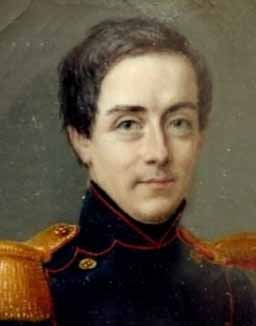
\includegraphics{complex/figures/pierre_laurent}
  \caption{Pierre Alphonse Laurent (1813–1854)}
\end{marginfigure}

This generalisation of a Taylor series in the presence of singularities is called a \emph{Laurent series}, in this case a Laurent series around the origin.


As an example, let's develop

$$f(z)=\frac{1}{z(z-1)}$$

in a Laurent series around the origin for the two rings $0 < | z | < 1$ and $ 1 < |z|$.

\begin{cue}
Do this first for the region where  $| z | < 1$, using the geometric series.
\end{cue}

For the first ring where $| z | < 1$, we can easily write

$$f(z)=\frac{1}{z} \cdot \frac{1}{z-1} = -\frac{1}{z} \sum_{m=0}^{\infty} z^m =-\frac{1}{z}-1-z-z^2 \cdots$$

However, in the second ring  $ 1 < |z|$, the previous series does not converge.

\begin{cue}
Divide the numerator and denominator of $f(z)$ by $z$, such that you can use the geometric series again.
\end{cue}

We can write

$$f(z)=\frac{1}{z} \cdot \frac{1 / z }{1-1/z} = \frac{1}{z^2} \sum_{m=0}^{\infty} \frac{1}{z^m} =\cdots+\frac{1}{z^4}+\frac{1}{z^3} + \frac{1}{z^2}$$

This series converges in the second ring, since $|1/z| < 1$ there.

\begin{exer}
% difficulty: normal
% ugent
\label{ex_laurent_1}
Develop

$$f(z)=\frac{e^z}{z-1}$$

in a Laurent series around the origin for the ring $0 < | z | < 1$.

$e^z$ is a function which is analytic in all of $\mathbb{C}$ and defined by

$$e^z \stackrel{def}{=} \sum_{m=0}^{\infty} \frac{z^m}{m!} $$

Can you also think of a graphical representation that helps you take the product of the two series expansions? (It's helpful to look at the solution video here.)

\begin{sol}
$$f(z)= - \sum_{k=0}^{\infty} \left(\sum _{m=0}^k \frac{1}{m!} \right) z^k $$
\end{sol}

\end{exer}

\begin{exer}
% difficulty: normal
  Same as Exercise \ref{ex_laurent_1}, but for the outer ring  $1 < | z |$.

\begin{sol}
$$f(z)=  \sum_{k=-\infty}^{\infty} \left(\sum_{m=k+1}^\infty \frac{1}{m!} \right) z^k $$
\end{sol}
  
\end{exer}

\begin{exer}
  % difficulty: normal
  Show that the exact location of the contours to derive Laurent series does not matter, as long as the contours don't cross any singularities.

\end{exer}

\begin{exer}
  % difficulty: hard
  What is the relationship between a Fourier and a Laurent series?
  \begin{hnt}
  Transform a Fourier series in exponential notation to a Laurent series.
  \end{hnt}
\end{exer}


\pagebreak


\sectionugent{Singularities}

$z_0$ is a singular point of $f(z)$ if $f(z)$ is not analytic there. There are two important types of singularities, \emph{poles} and \emph{branch points}, which we will now discuss.

\subsection*{Poles}

We develop $f(z)$ in a Laurent series around $z_0$:

\begin{equation}
f(z)= \sum_{m=-\infty}^{\infty} a_m (z-z_0)^m
\end{equation} 

If the index $m$ doesn't run all the way to $-\infty$, but only to a finite value $-M$, $z_0$ is called a \emph{pole of order $M$}. As a trivial example, $f(z)=1/z$ has a pole of order 1 at $z=0$ (also called a \emph{simple pole}). $f(z)=1/z^2$ has a pole of order 2 at $z=0$

On the other hand, if there is an infinite number of negative $m$--values for which $a_m$ is non--zero, $z_0$ is called an \emph{essential singularity}.

\begin{cue}
  Verify by looking at the series expansion that $f(z)=e^{1/z}$ is an essential singularity.  
\end{cue}

Since

$$e^{1/z} = \sum_{m=0}^{\infty} \frac{1}{z^m m!} $$

has an infinite number of negative powers of $z$, it is an essential singularity.

Note that a pole of order $M$ can be removed by multiplying $f(z)$ by $(z-z_0)^M$. This obviously cannot be done for an essential singularity.

\noindent\marginnote{This is shown in Picard's Great Theorem.}One can also prove that in a small neighbourhood around an essential singularity, the function actually takes all possible complex values (with at most a single exception)! So, obviously it makes no sense to talk about the limit of that function there.

\pagebreak

\subsection*{Branch points}

Consider the relation

\begin{equation}
w = f(z) = z^{1/2} \label{eq-sqrt}
\end{equation}

(As a notational oddity, the complex square root is designated by the power $1/2$, to distinguish it from the real-valued square root.)

\begin{cue}
For a given value of $z$, how many solutions $w$ does the complex square root have? 
\end{cue}

For $z=\rho e^{j\theta}$, a possible solution to Eq.~\ref{eq-sqrt} is $w_1 = \rho^{1/2} e^{j\theta/2}$. However, there is a different point in the $w$--plane that corresponds to the same $z$, namely $w_2 = \rho^{1/2} e^{j(\theta/2+\pi)} = -w_1$. This is the complex analog of the real equation $y^2 = x$ for $x > 0$, which has two solutions $y = \pm \sqrt{x}$.

So, Eq.~\ref{eq-sqrt} is clearly not a single--valued function: a single point in the $z$--plane (except $z=0$) corresponds to two points in the $w$--plane. To get a handle on the multivaluedness of $z^{1/2}$, it's instructive to look at a graphical representation of this complex function. Since this is essentially a 4D--object, we can plot e.g. a 3D projection $(\Re(z),\Im(z),\Re(w))$ and use the phase of $w$ to colour the surface. This is done in Fig.~\ref{fig-riemann}.

\begin{marginfigure}[-3cm]
\centering
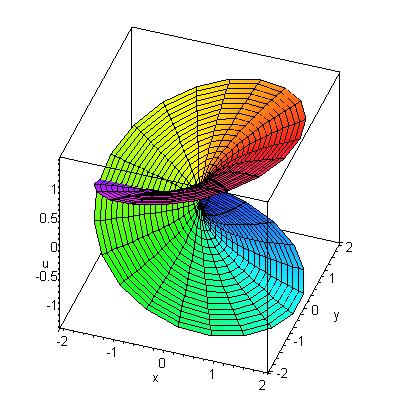
\includegraphics{complex/figures/riemann}
\caption{Riemann surface of $w=z^{1/2}$. Note that $u=\Re(w)$. }
\label{fig-riemann}
\end{marginfigure}

This 4D--object is also called the \emph{Riemann surface} of the complex square root function and Fig.~\ref{fig-riemann} shows a representation of it. It clearly shows the multivaluedness of the square root: for each point in the $z$--plane there are two points on the Riemann surface. Another way to appreciate this multivaluedness is by looking at how the argument of $w$ changes if we pick a point on the surface, make a full round trip on the Riemann surface, and arrive back at our original point.

\begin{cue}
When you do such an excursion in the complex plane, how does the angle of $w$ change? 
\end{cue}

From the figure, it is clear that we will have circled twice around the origin for that, so one could say that on the Riemann surface, the argument $w$ needs to change over $4 \pi$ in order to complete a full round trip. Therefore, this Riemann surface can be seen as an extension of the complex plane which is 'twice as large' as the regular complex plane.

Although the Riemann surface is a very profound and beautiful mathematical concept, for practical purposes people often like to work with single--valued functions mapping the complex plane to the regular (i.e. non-extended) complex plane. To do this, we can adopt a convention to restrict ourselves e.g. to values in the right half of the $w$--plane, i.e. where $\Re(w)>0$.


\begin{marginfigure}[-1cm]
\centering
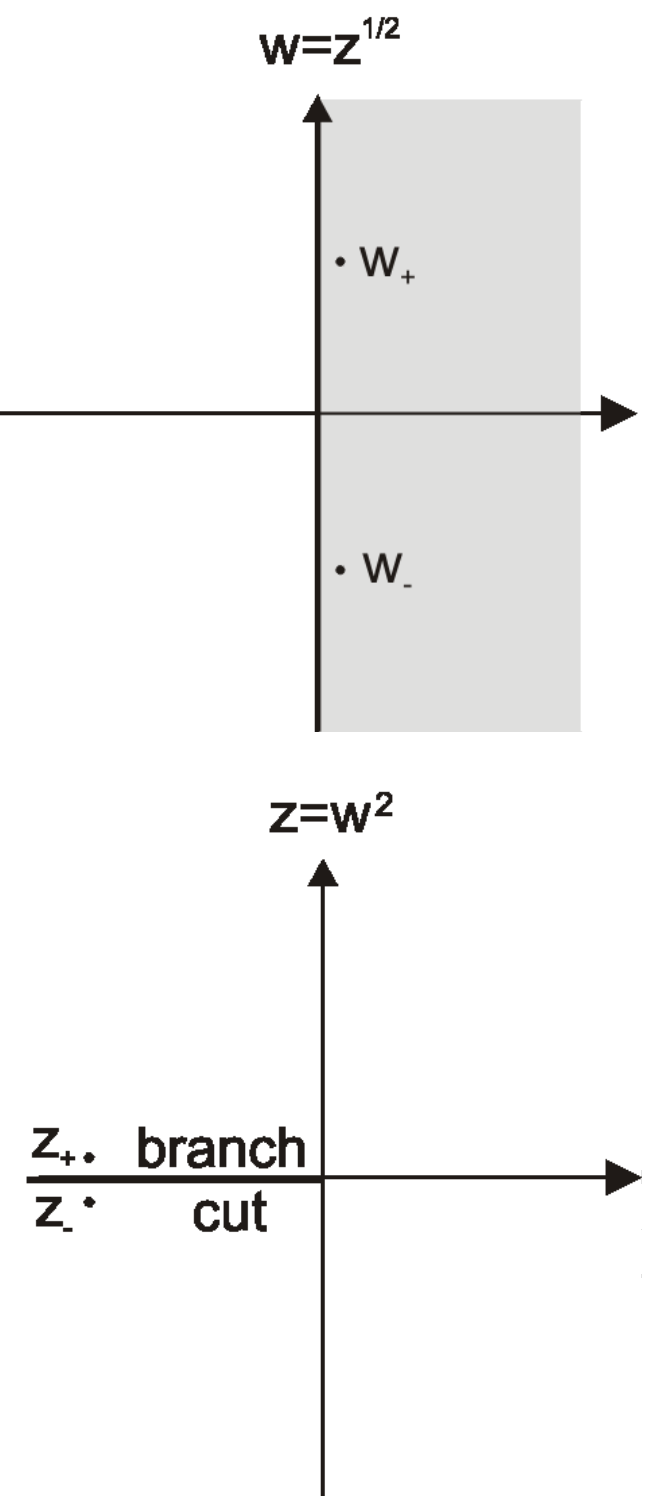
\includegraphics[width=4cm]{complex/figures/branchcut_portrait}
\caption{The mapping $w=z^{1/2}$.}
\label{fig-branchcut}
\end{marginfigure}


\begin{cue}
To which figure in the $z$--plane does the boundary $\Re(w)=0$ map?
\end{cue}

The boundary $\Re(w)=0$ between these two halves of the $w$--plane corresponds to the negative real axis in the $z$--plane. We call this negative real $z$--axis a \emph{branch cut}, originating from the \emph{branch point} $z=0$ (see Fig.~\ref{fig-branchcut}).

\begin{cue}
Looking at Fig.~\ref{fig-branchcut}, once we introduce the branch cut, what is the square root of $z_+$ and $z_-$? What happens to the output of the function if you cross the branch cut in the $z$--plane? 
\end{cue}

Our function is now no longer continuous when crossing the branch cut: for $z_+ = \rho e^{j (\pi - \epsilon)}$, we get $w_+ = \sqrt{\rho} e^{j (\pi/2 - \epsilon/2)}$, whereas for $z_- = \rho e^{j (\pi + \epsilon)}$, we get $w_- = \sqrt{\rho} e^{j (\pi/2 + \epsilon/2)} e^{j \pi}$. (This can be seen by looking at Fig.~\ref{fig-branchcut}.) In the limit of zero $\epsilon$, $w_+$ tends to $j\sqrt{\rho}$, whereas $w_-$ tends to $-j\sqrt{\rho}$.

\begin{marginfigure}[1cm]
\centering
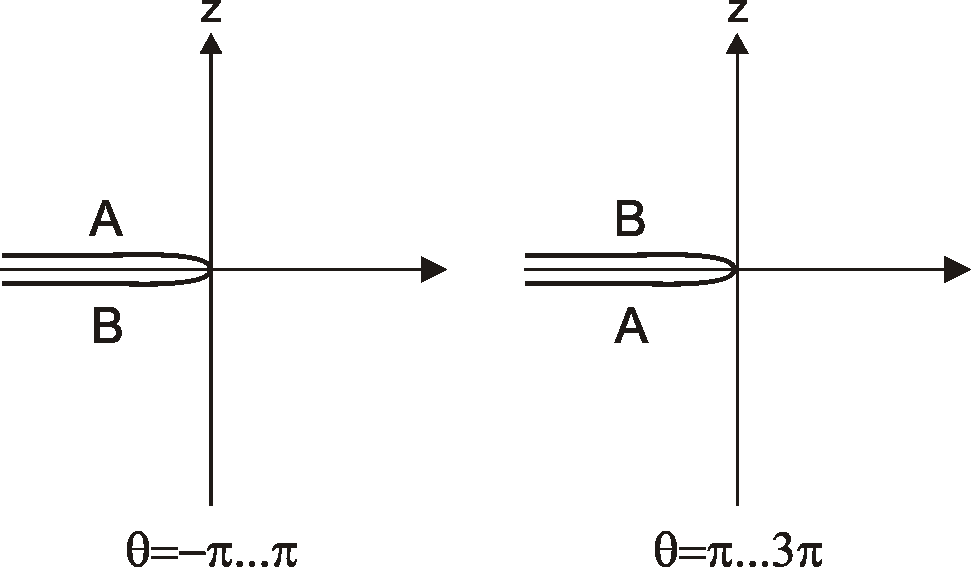
\includegraphics{complex/figures/sheets}
\caption{The branch cut cuts the Riemann surface in two separate Riemann sheets.
Adjacent regions on the Riemann surface are marked by the same letters.}
\label{fig-sheets}
\end{marginfigure}

The relationship between branch cuts and the Riemann surface is show schematically in Fig.~\ref{fig-sheets}: our branch cut cuts the Riemann surface in two separate \emph{Riemann sheets}, one corresponding to arguments $[-\pi, \pi]$, the other one corresponding to arguments $[\pi,3 \pi]$.

It is important to remark that, when choosing a contour to evaluate the integral theorems we've seen so far, we are not allowed to cross a branch cut, as the resulting discontinuity would make the function no longer analytic. However, skirting on one edge of a branch cut, circling around the branch point and returning along the other edge is allowed, as the function stays continuous and analytic throughout the entire path. 

Note that integrals on both sides of a branch cut will generally not cancel out, unlike integrals on both sides of the contour cut in Fig.~\ref{fig-cauchy-II}, which only serves to transform a contour into one which can be used to apply Cauchy's theorem.

The choice of branch cut is in no way unique: any line (even a curved one) from $z=0$ to infinity would suit the purpose equally well. Its only goal is to lift the ambiguity with respect to the choice of $w$. There are however often physical reasons which inspire the choice of branch cut.

\pagebreak

\begin{exer}
% difficulty: normal
% ugent
\label{ex-branch-ang}
Show that asking that $\Re(w)>0$ is equivalent to asking that you restrict the angle of $z$ to $[-\pi, \pi]$ before halving it to calculate the square root. Do this by looking at 4 strategically located points in the $z$-plane (just above/below the positive/negative real axis). Write down their angles, and then see what the corresponding angles in the $w$--plane are. Are the results in the correct half plane? Verify that crossing the branch cut leads to a discontinuity. 
\end{exer}

\begin{exer}
% difficulty: normal
% ugent
  \label{ex-product-roots}
\begin{marginfigure}[0.5cm]
\centering
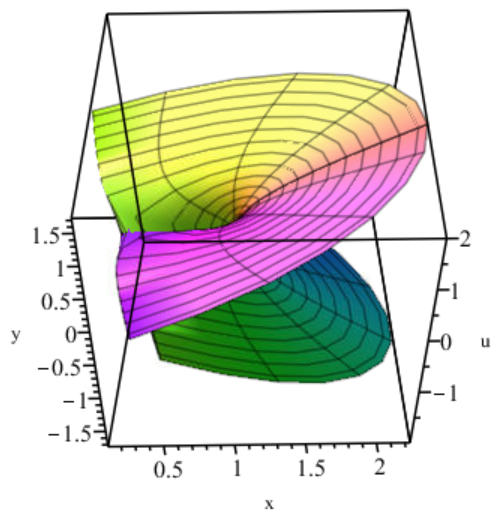
\includegraphics[width=4cm]{complex/figures/riemann2}
\caption{Half the Riemann surface of $w=(z-1)^{1/2}(z+1)^{1/2}$. Note that $u=\Re(w)$. }
\label{fig-riemann2}
\end{marginfigure}
Consider

$$f(z)=(z-1)^{1/2}(z+1)^{1/2}$$

Using the conventional choice of branch cut for an individual square root (expressed in terms of angles as in Ex.~\ref{ex-branch-ang}), show that the branch cut for this product of square roots is the segment $-1 \le x \le 1$. Do this by looking at 8 strategically located points in the $z$--plane, and calculate the angle of the corresponding $w$--value.


Verify that it is possible to establish a single--valued function using this cut, and that any contour which does not cross this cut does not encounter discontinuities.
\end{exer}

\begin{exer}
% difficulty: normal
What does the Riemann surface of $w=\ln(z)$ look like?
\end{exer}

\begin{exer}
% difficulty: hard
\begin{marginfigure}[0.cm]
\centering
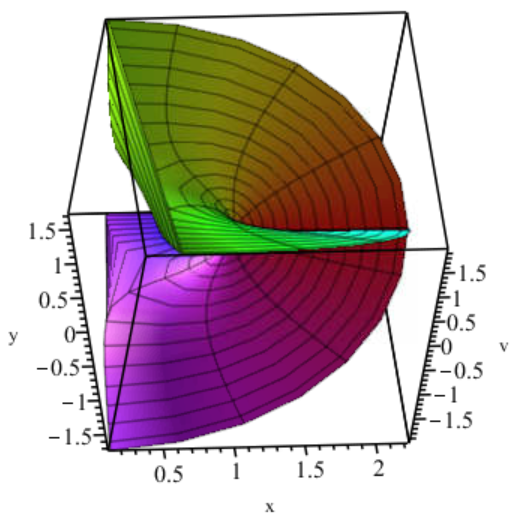
\includegraphics[width=4cm]{complex/figures/riemann3}
\caption{Half the Riemann surface of $w=(z-1)^{1/2}(z+1)^{1/2}$. Note that $v=\Im(w)$. }
\label{fig-riemann3}
\end{marginfigure}

For Eq.~\ref{ex-product-roots}, what range of angles would you need to chose for the arguments of each of the square roots in order to end up with a branch cut consisting of the union of  $x \le -1$ and $1 \le x$?


Note that Fig.~\ref{fig-riemann2} and \ref{fig-riemann3} each seem to suggest a different natural choice for a branchut, even though they both correspond to the same Riemann surface.


Why is that? Which branch cut is more natural?
  \begin{sol}
    $\arg(z-1) \in [0, 2 \pi], \arg(z+1) \in [-\pi,\pi]$. Figs.~\ref{fig-riemann2} and \ref{fig-riemann3} are both different projections of a 4D Riemann surface. That they seem to suggest a certain natural choice for the branchcut is purely accidental.
\end{sol}
\end{exer}

\pagebreak


\sectionugent{Residue calculus}

One of the main goals of this chapter is to provide you with a powerful way of calculating some real-valued integrals by transforming them to complex contour integrals, and solve them using straightforward algebra, as opposed to using tricky calculus. An important ingredient in this recipe is the use of so-called \emph{residue calculus}.

\subsection*{Residue}

Suppose $z_0$ is an isolated singularity of $f(z)$. We can develop this function in a Laurent series around $z_0$:

\begin{equation}
f(z)= \sum_{m=-\infty}^{\infty} a_m (z-z_0)^m
\end{equation} 

The \emph{residue} of $z_0$ is defined as $a_{-1}$, i.e. the coefficient of $1/z$ in the Laurent series. Using Eq.~\ref{eq-laurent-int}, we immediately get

\begin{equation}
\mathrm{Res}_{z_0}=\frac{1}{2 \pi j }  \oint_{{C}} f(z) dz \label{eq-res-int}
\end{equation}

\begin{cue}
  By looking at their series expansion, calculate the residues of the following functions at $z=0$.
  $$\begin{array}{lcll}a) & f(z)=1/z \\b) & f(z)=1/z^2 \\c) & f(z)=e^{1/z}\end{array}$$
\end{cue}

For $f(z)=1/z$ and $f(z)=1/z^2$, the series expansion is the function itself, so we can quickly see that the residues are 1 and 0 respectively.

$z=0$ is an essential singularity of $f(z)=e^{1/z}$ with residue 1, since

$$e^{1/z} = \sum_{m=0}^{\infty} \frac{1}{z^m m!} $$

\begin{exer}
% difficulty: trivial
  Integrate the Laurent series around a singularity term-by-term. What formula do you recover?
\end{exer}

\begin{exer}
% difficulty: normal
  Use a series expansion to calculate the residue at $z=0$ of
  $$z \cos \frac{1}{z}$$
  \begin{sol}
    $$-1/2$$
  \end{sol}
\end{exer}

\begin{exer}
% difficulty: normal
  Use a series expansion to calculate the residue at $z=0$ of

  $$\frac{z - \sin z}{z}$$
  \begin{sol}
    $$0$$
  \end{sol}
\end{exer}


\subsection*{Residue theorem}

Suppose $f(z)$ is analytic inside a contour ${C}$, except for some isolated singularities $z_k$ inside ${C}$ (so, branch cuts are not allowed, but e.g. poles are OK). Then

\begin{equation}
\fbox{$\displaystyle
\oint_{{C}} f(z) dz = 2 \pi j \sum_k \mathrm{Res}_{z_k} \label{eq-res-theorem}
$}
\end{equation} 

The summation index $k$ runs over all singularities enclosed by the contour. Note that no singularity should lie on the contour itself.

\begin{marginfigure}
\centering
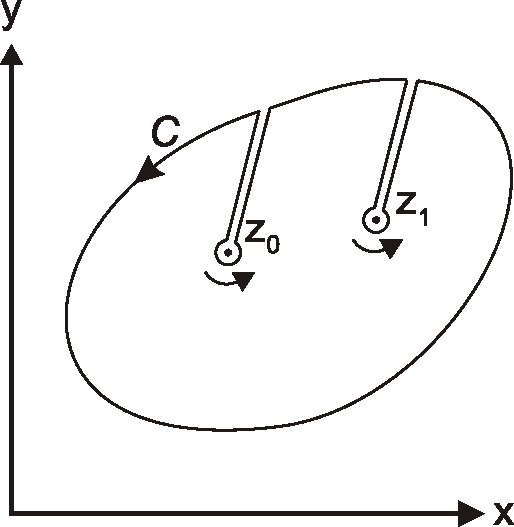
\includegraphics{complex/figures/residue}
\caption{Contour to prove residue theorem.}
\label{fig-residue}
\end{marginfigure}

To prove Eq.~\ref{eq-res-theorem}, we make use of the contour in Fig.~\ref{fig-residue}.

\begin{cue}
  Apply Cauchy's theorem on this contour. Then, use the relation between the residue and a contour integral around the singularity (Eq.~\ref{eq-res-int}) to prove the residue theorem. 
\end{cue}

Applying Cauchy's theorem on this contour (the straight segments cancel as before):

\begin{equation}
\oint_{{C}} f(z) dz - \sum_k \oint_{{C}_k} f(z) dz = 0
\label{eq-res-proof-1}
\end{equation}

The integral around any singular point can be written as (Eq.~\ref{eq-res-int})

\begin{equation}
\oint_{{C}_k} f(z) dz = 2 \pi j \mathrm{Res}_{z_k} \label{eq-res-proof-2}
\end{equation} 

Combining Eq.~\ref{eq-res-proof-1} and Eq.~\ref{eq-res-proof-2} immediately proves the theorem.

\subsection*{Calculating residues}

The residue theorem is of enormous practical importance, as it allows us to replace the cumbersome problem of evaluating contour integrals by the algebraic problem of calculating residues at enclosed singular points. Because of its importance, we will now discuss a number of techniques that allow us to easily calculate the residues, apart from writing down the Laurent series, or applying Eq.~\ref{eq-res-int}. The proofs are left as an exercise. The formulas for the case of a single pole are worth memorising.

\begin{exer}
% difficulty: normal
% ugent
  If $z_0$ is a simple pole of $f(z)$, use the Laurent series to prove that
  $$\mathrm{Res}_{z_0} = \left[f(z)(z-z_0)\right]_{z=z_0}$$

  (Explicitly writing down the first few terms of the Laurent series makes this slightly easier to solve.)
  
\label{ex-res1}
\end{exer}

\begin{exer}
% difficulty: trivial
  Calculate the residue at $z=0$ of

   $$\frac{1}{z+z^2}$$ 
\begin{sol}
  $$1$$
\end{sol}
\end{exer}

\begin{exer}
% difficulty: hard
% ugent
  If $z_0$ is a simple pole of $f(z)=\frac{g(z)}{h(z)}$, i.e. $z_0$ is a simple zero of $h(z)$ and $g(z_0) \ne 0$, show that
    $$\mathrm{Res}_{z_0} = \frac{g(z_0)}{h'(z_0)}$$
\begin{hnt}
Write $h(z)$ as $r(z)(z-z_0)$, and apply the result from Ex.~\ref{ex-res1}.
\end{hnt}
\end{exer}

\begin{exer}
% difficulty: hard
If $z_0$ is a pole of order $M$ of $f(z)$, prove that
$$\mathrm{Res}_{z_0} = \frac{1}{(M-1)!}{\left[D^{M-1}[f(z)(z-z_0)^M]\right]}_{z=z_0}$$
\end{exer}


\pagebreak


\sectionugent{Limit theorems}

Sometimes, we are dealing with contours that are infinitely large or infinitely small. For these cases, the following limit theorems (which we will present mostly without proof) are of great practical importance.

\subsection*{Jordan's lemma}

\begin{marginfigure}
\centering
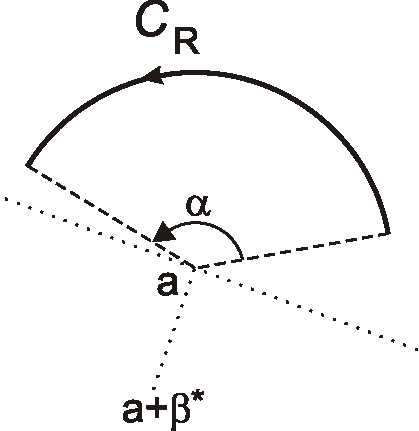
\includegraphics[width=4cm]{complex/figures/jordan}
\caption{Jordan's lemma.}
\label{fig-jordan}
\end{marginfigure}

Jordan's lemma deals with integrals along a circular path  (see Fig.~\ref{fig-jordan}) containing a complex exponential: 

$$ \int_{{C}_R} f(z) e^{\beta z} dz$$

Note that here (and also for the next limit theorems) ${{C}_R}$ only includes the circular part of the contour and not the straight line segments.

Under which circumstances does this integral go to zero if the radius $R$ goes to infinity? It seems reasonably that both factors of the integrand should go to zero for that. However, the exponential does not go to zero at infinity everywhere in the complex plane. 

\begin{cue}
Show that if $b>0$, then $e^{jbz}$ goes to zero if $z$ goes to infinity, but only in the upper half plane.
\end{cue}

It can be shown that in general, for a contour lying on the 'proper' side of $a$, i.e. the half plane not containing $a+\beta^*$ (see Fig.~\ref{fig-jordan}), we have that if

\begin{marginfigure}[-2.5cm]
  % credits: Wikipedia
  % url: https://en.wikipedia.org/wiki/Camille_Jordan
  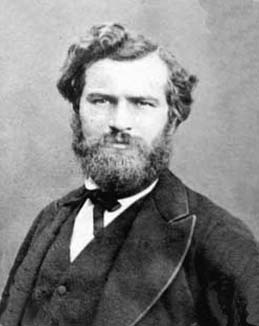
\includegraphics{complex/figures/camille_jordan}
  \caption{Camille Jordan (1838–1922) }
\end{marginfigure}

\begin{equation}
\lim_{z \to \infty} f(z) = 0
\end{equation}
then
\begin{equation}
\lim_{R \to \infty} \int_{{C}_R} f(z) e^{\beta z} dz = 0
\end{equation}

\begin{cue}
Verify that the construction of the 'proper' half plane reduces to the upper half plane in case $a=0$ for $ \int_{{C}_R} f(z) e^{jb z} dz$ with $b>0$.
\end{cue}

\subsection*{Big limit theorem}

For a circular contour spanning an angle $\alpha$ with top at $z=a$ (see Fig.~\ref{fig-limit-theorem}), we have that if

\begin{equation}
\lim_{z \to \infty}  f(z) (z-a) = A
\end{equation}
then
\begin{equation}
\lim_{R \to \infty} \int_{{C}_R} f(z) dz = j \alpha A
\end{equation}

\begin{marginfigure}
\centering
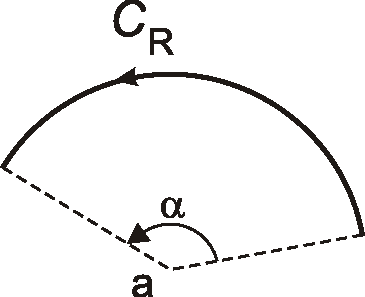
\includegraphics[width=3.5cm]{complex/figures/limit_theorem}
\caption{Contours for big and small limit theorems.}
\label{fig-limit-theorem}
\end{marginfigure}

Important: do not confuse when to use Jordan's lemma and when to use the big limit theorem (look for the presence of an exponential). Also do not confuse when to add a factor $z-a$ to the limit related to $f(z)$.

\subsection*{Small limit theorem} 

For a circular contour spanning an angle $\alpha$ with top at $z=a$ (see Fig.~\ref{fig-limit-theorem}), we have that if

\begin{equation}
\lim_{z \to a}  f(z) (z-a) = A
\end{equation}
then
\begin{equation}
\lim_{R \to 0} \int_{{C}_R} f(z) dz = j \alpha A
\end{equation}

\begin{exer}
  % difficulty: hard
  Prove the small limit theorem for the special case where $f(z)$ has a single pole at $z=a$.
  \begin{hnt}
    Integrate the Laurent series term by term.
  \end{hnt}
\end{exer}

\subsection*{Cauchy principal value}

\begin{marginfigure}
\centering
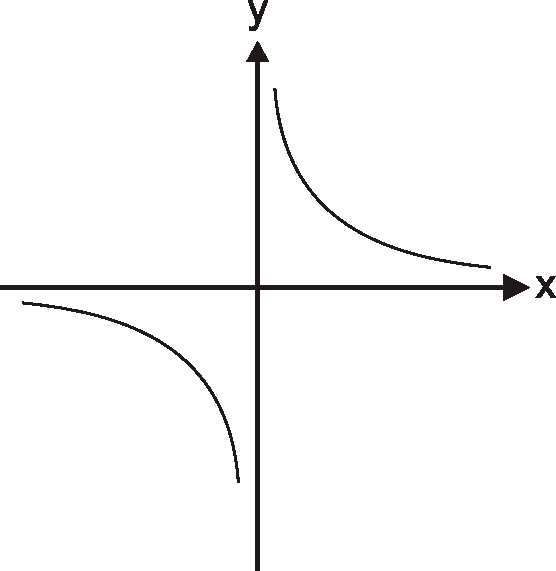
\includegraphics[width=4cm]{complex/figures/pv}
\caption{The function $1/x$.}
\label{fig-pv}
\end{marginfigure}

Let's discuss a final technicality that will come handy in some cases. Consider the integral $\int_0^1 dx / x$ (see Fig.~\ref{fig-pv}). As the area under this curve is infinite, this integral clearly diverges.

Strictly speaking, the same is true for the integral $\int_{-1}^1 dx / x$, as this should be seen as

\begin{equation}
\lim_{\epsilon_1 \to 0} \int_{-1}^{-\epsilon_1} \frac{dx}{x} + \lim_{\epsilon_2
\to 0} \int_{\epsilon_2}^1 \frac{dx}{x}
\end{equation}  

because each term separately diverges, and the limits are taken independently. However, Fig.~\ref{fig-pv} suggests that both singularities will cancel out. Mathematically, this means that

\begin{equation}
\lim_{\epsilon \to 0} \int_{-1}^{-\epsilon} \frac{dx}{x} + \lim_{\epsilon \to 0}
\int_{\epsilon}^1 \frac{dx}{x} = 0 \label{eq-pv}
\end{equation}  

if both limits are taken at the same time. This is written succinctly as

\begin{equation}
PV \int_{-1}^1 \frac{dx}{x} = 0
\end{equation} 

where $PV$ stands for the Cauchy \emph{principal value} and represents the balancing process of Eq.~\ref{eq-pv}. However, $\int_{-1}^1 dx / x$ still diverges.

The same balancing process can also be applied to limits at infinity:

\begin{equation}
PV \int_{-\infty}^\infty f(x) dx = \lim_{a \to \infty} \int_{-a}^{a} f(x) dx
\end{equation} 

\pagebreak

\sectionugent{Evaluation of real--valued integrals}

Now we have all the necessary tools in our box to tackle the important problem
of calculating real--valued integrals by means of complex contour integration.
We will present a number of examples which illustrate some typical techniques
used in this respect.

\subsection*{Example 1: integrals of the type $\int_0^{2 \pi} f(\cos \theta, \sin \theta) d \theta$}

Consider integrals of the type

\begin{equation}
\int_0^{2 \pi} f(\cos \theta, \sin \theta) d \theta \label{eq-cont-int-1}
\end{equation} 

By letting $z=e^{j \theta}$, we get 

\begin{equation}
\cos \theta = \frac{z + 1/z}{2}
\end{equation} 

\begin{equation}
\sin \theta = \frac{z - 1/z}{2j}
\end{equation} 

\begin{equation}
d \theta = \frac{1}{j}\frac{dz}{z}
\end{equation} 

such that the integral Eq.~\ref{eq-cont-int-1} becomes

\begin{equation}
-j \oint_{{C}} f\left(\frac{z + 1/z}{2}, \frac{z - 1/z}{2j}\right)
\frac{dz}{z}
\end{equation} 

The integration contour ${C}$ is the unit circle, and the integral can easily be evaluated using the residue theorem.

As an example, we will calculate

\begin{equation}
I = \int_0^{2 \pi} \frac{d \theta}{1 + \epsilon \cos \theta}, \hspace{0.5cm}
|\epsilon| < 1
\end{equation} 

\begin{cue}
  Transform this to a complex contour integral.
\end{cue}

This transforms into

\begin{equation}
I = -j \oint_{{C}} \frac{1}{1 + (\epsilon / 2)\left(z + 1/z\right)}
\frac{dz}{z}
\end{equation} 

or

\begin{equation}
I = -\frac{2j}{\epsilon} \oint_{{C}} \frac{dz}{z^2 + (2 / \epsilon)z +
1}
\end{equation} 

\begin{cue}
  Where are the poles of this function? Calculate the relevant residues.
\end{cue}

The poles of this function are

\begin{equation}
z = - \frac{1}{\epsilon} \pm \frac{1}{\epsilon} \sqrt{1 - \epsilon^2}
\end{equation} 

Only the pole with the plus sign lies within the unit circle, as can be verified e.g. by a series expansion for small values of $\epsilon$. By using the formula from Ex. \ref{ex-res1} to calculate the residue there, we get

\begin{equation}
I = -\frac{2j}{\epsilon} \cdot 2 \pi j \left[\frac{1}{z - (-\frac{1}{\epsilon} -
\frac{1}{\epsilon} \sqrt{1 - \epsilon^2})}\right]_{z = - \frac{1}{\epsilon} +
\frac{1}{\epsilon} \sqrt{1 - \epsilon^2}}
\end{equation}

or

\begin{equation}
I = -\frac{2j}{\epsilon} \cdot 2 \pi j \cdot \frac{1}{\frac{2}{\epsilon} \sqrt{1
- \epsilon^2}}
\end{equation}

\begin{cue}
  Combine everything to calculate the original integral.
\end{cue}

So finally

\begin{equation}
\int_0^{2 \pi} \frac{d \theta}{1 + \epsilon \cos \theta} = \frac{2 \pi}{\sqrt{1
- \epsilon^2}}, \hspace{0.5cm} |\epsilon| < 1
\end{equation} 

\pagebreak
\subsection*{Example 2: integrals of the type $\int_\infty^{\infty} f(z) e^{jbz} dz$}

Let's calculate

\begin{equation}
\int_0^{\infty}\frac{\cos \lambda x}{1 + x^2} dx, \hspace{0.5cm} \lambda > 0
\end{equation}

\noindent\marginnote{Alternatively, we could have made use of $\cos z = (e^{j z} + e^{-jz})/2$, but then Jordan's lemma would have required two separate integrals for each of the complex exponentials, each with a different contour.}To do this, we will calculate the real part of the following contour integral (Fig.~\ref{fig-example-2}):

\begin{equation}
I = \oint_{{C}} \frac{e^{j \lambda z}}{1 + z^2} dz
\end{equation}

\begin{marginfigure}
\centering
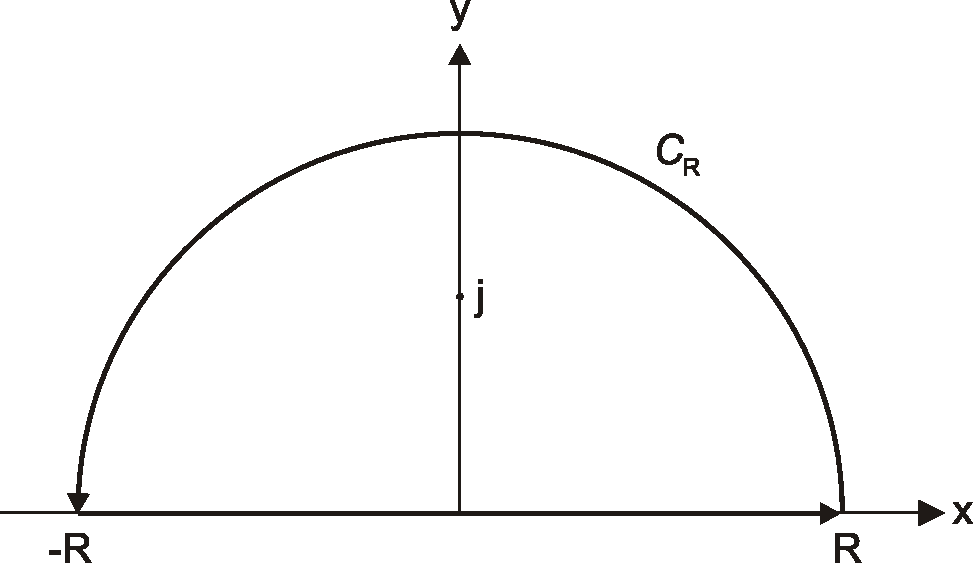
\includegraphics{complex/figures/int_ex_2}
\caption{Contour for example 2.}
\label{fig-example-2}
\end{marginfigure}

Evaluating the part of this contour on the positive real axis, and then taking the real part will recover the required cosine in the integral. It is true that we are only interested in the contribution from the positive real axis, but as you'll see, we'll be able to deal with the other contributions in due course.

\begin{cue}
Use residue calculus to evaluate the contour integral.
\end{cue}

The only pole enclosed by the contour is at $j$, with residue $e^{-\lambda}/(j+j)$, such that the residue theorem leads to

\begin{equation}
\int_{-R}^{R} \frac{e^{j \lambda x}}{1 + x^2} dx + \int_{{C_R}}
\frac{e^{j \lambda z}}{1 + z^2} dz = 2 \pi j \frac{e^{-\lambda}}{2 j} = \pi
e^{-\lambda}
\end{equation}

Let's now take the limit $R \to \infty$ and study the different contributions to the contour.

\begin{cue}
Can we apply Jordan's lemma to ${C_R}$? 
\end{cue}

If $\lambda > 0$, the contour lies indeed in the 'proper' part of the complex plane. For the second condition, we need to calculate the following limit:

\begin{equation}
\lim_{z \to \infty}\frac{1}{1+z^2} = \lim_{z \to \infty}\frac{1}{1+|z|^2 e^{2 j
\arg z}}
\end{equation}

Since $e^{2 j \arg z}$ always stays bounded, this limit goes to zero for all directions in the complex plane. So, we can apply Jordan's lemma and the contribution from ${C_R}$ vanishes.

\begin{cue}
Write down what remains of the contour integral and use this to calculate our original real-valued integral.
\end{cue}

\begin{equation}
\int_{-\infty}^{\infty}\frac{e^{j \lambda x}}{1 + x^2} dx = \pi e^{-\lambda}
\end{equation}

\noindent\marginnote{Only for readers that like to lie awake at night about mathematical rigour: strictly speaking, you should take the real part \emph{before} taking the limit $R \to \infty$. Can you see why?}After taking the real part of the result, we get

\begin{equation}
\int_{-\infty}^{\infty}\frac{\cos \lambda x}{1 + x^2} dx = \pi e^{-\lambda}
\end{equation}

Finally, due to the even character of the integrand, we arrive at

\begin{equation}
\int_0^{\infty}\frac{\cos \lambda x}{1 + x^2} dx = \frac{\pi}{2} e^{-\lambda}
\end{equation}

\subsection*{Example 3: integrals with branch cuts}

Let's now try an example with branch point singularities:

\begin{equation}
\int_0^{\infty}\frac{\sqrt{x}}{x^2+a^2}dx, \hspace{0.5cm} a > 0
\end{equation}

\begin{marginfigure}[-0cm]
\centering
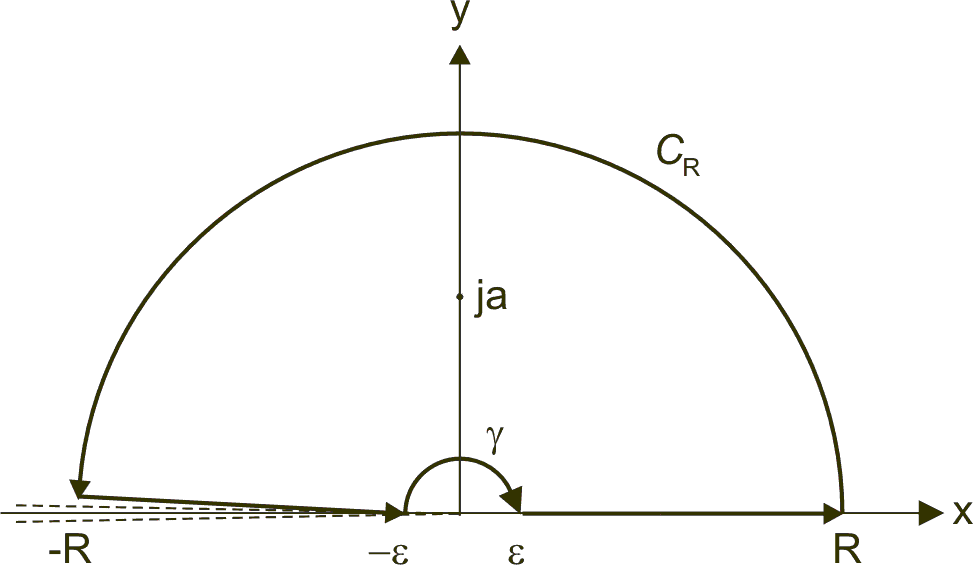
\includegraphics{complex/figures/int_ex_3}
\caption{Contour for example 3.}
\label{fig-example-3}
\end{marginfigure}

We stick to the traditional choice of branch cut, namely the negative real axis (Fig.~\ref{fig-example-3}). The contour is placed 'just above' this branch cut. In order to avoid the branch point at $z=0$, we also make a small detour around the origin.

\begin{cue}
Use residue calculus to evaluate the contour integral.
\end{cue}

\begin{align}
I = \oint_{{C}} \frac{z^{1/2}}{z^2+a^2} dz =& \, 2 \pi j \textrm{Res}_{j a}
\nonumber \\
=& \, 2 \pi j \frac{(j a)^{1/2}}{ja + ja} \nonumber \\
=& \, \pi \frac{\sqrt{a}e^{\frac{1}{2}j\frac{\pi}{2}}}{a} \nonumber \\
=& \, \frac{\pi}{\sqrt{a}} e^{j \pi /4}
\end{align}

\begin{cue}
What is the contribution of ${C_R}$ to the integral in the limit of infinite radius?
\end{cue}

We use the big limit theorem to calculate the contribution of the outer circular part ${C_R}$ to the integral. For that, we calculate the following limit:

\begin{equation}
\lim_{z \to \infty}\frac{z^{1/2}}{z^2+a^2} \cdot z = \lim_{z \to
\infty}\frac{\sqrt{|z|}e^{j \arg z / 2}}{|z|^2 e^{2 j \arg z}+a^2} \cdot |z|
e^{j \arg z}
\end{equation}

Just as before, the complex exponentials involving $\arg z$ always stay bounded, so this limit goes to zero and the contribution from this part of the contour vanishes.

\begin{cue}
What is the contribution of the small inner circle $\gamma$ to the integral in the limit of zero radius?
\end{cue}

Similarly, we use the small limit theorem to show that the contribution for the semicircle around the branch point vanishes in the limit of zero radius:

\begin{equation}
\lim_{z \to 0}\frac{z^{1/2}}{z^2+a^2} \cdot z = \frac{0}{a^2} = 0
\end{equation}

\begin{cue}
Write down what remains of the contour integral and use this to calculate our original real-valued integral.
\end{cue}

So finally we are left with

\begin{equation}
I = \int_{- \infty}^{0}\frac{z^{1/2}}{z^2+a^2}dz + \int_{0}^{\infty}\frac{z^{1/2}}{z^2+a^2}dz
\end{equation} 

Returning from $z$ to $x$, we get with our choice of branch cut (see the calculation of $w_+$ in the section on branch cuts) that 

\begin{equation}
z^{1/2} = 
\begin{cases}
\sqrt{x}, & x > 0\\
j \sqrt{-x}, & x < 0
\end{cases}
\end{equation} 

such that

\begin{align}
I = & \int_{- \infty}^{0}\frac{j\sqrt{-x}}{x^2+a^2}dx +
\int_{0}^{\infty}\frac{\sqrt{x}}{x^2+a^2}dx \nonumber \\
 = & \, (1 + j) \ \int_{0}^{\infty}\frac{\sqrt{x}}{x^2+a^2}dx \nonumber \\
 = & \, \frac{\pi}{\sqrt{a}} e^{j \pi /4}
\end{align} 

So finally

\begin{equation}
\int_0^{\infty}\frac{\sqrt{x}}{x^2+a^2}dx = \frac{\pi}{\sqrt{2a}}
\end{equation}

\pagebreak

\begin{exer}
% difficulty: trivial
% ugent
  \label{ex-contour-integral-1}
Use complex contour integration to calculate
$$\int_0^{\infty} \frac{dx}{1+x^2}$$
\begin{sol}
$$\frac{\pi}{2}$$
\end{sol}
\end{exer}

\begin{exer}
% difficulty: trivial
Repeat Ex.~\ref{ex-contour-integral-1}, but show that you get the same result if you close the contour in a different half plane, and/or change its orientation.
\end{exer}

\begin{exer}
% difficulty: trivial
% ugent
  Comment on the suitability of the following contours for calculating
  $$ \int_0^{\infty} \frac{\sin x}{x} dx$$

  (All of these were harvested from actual students trying their hand at this problem.)

\begin{center}
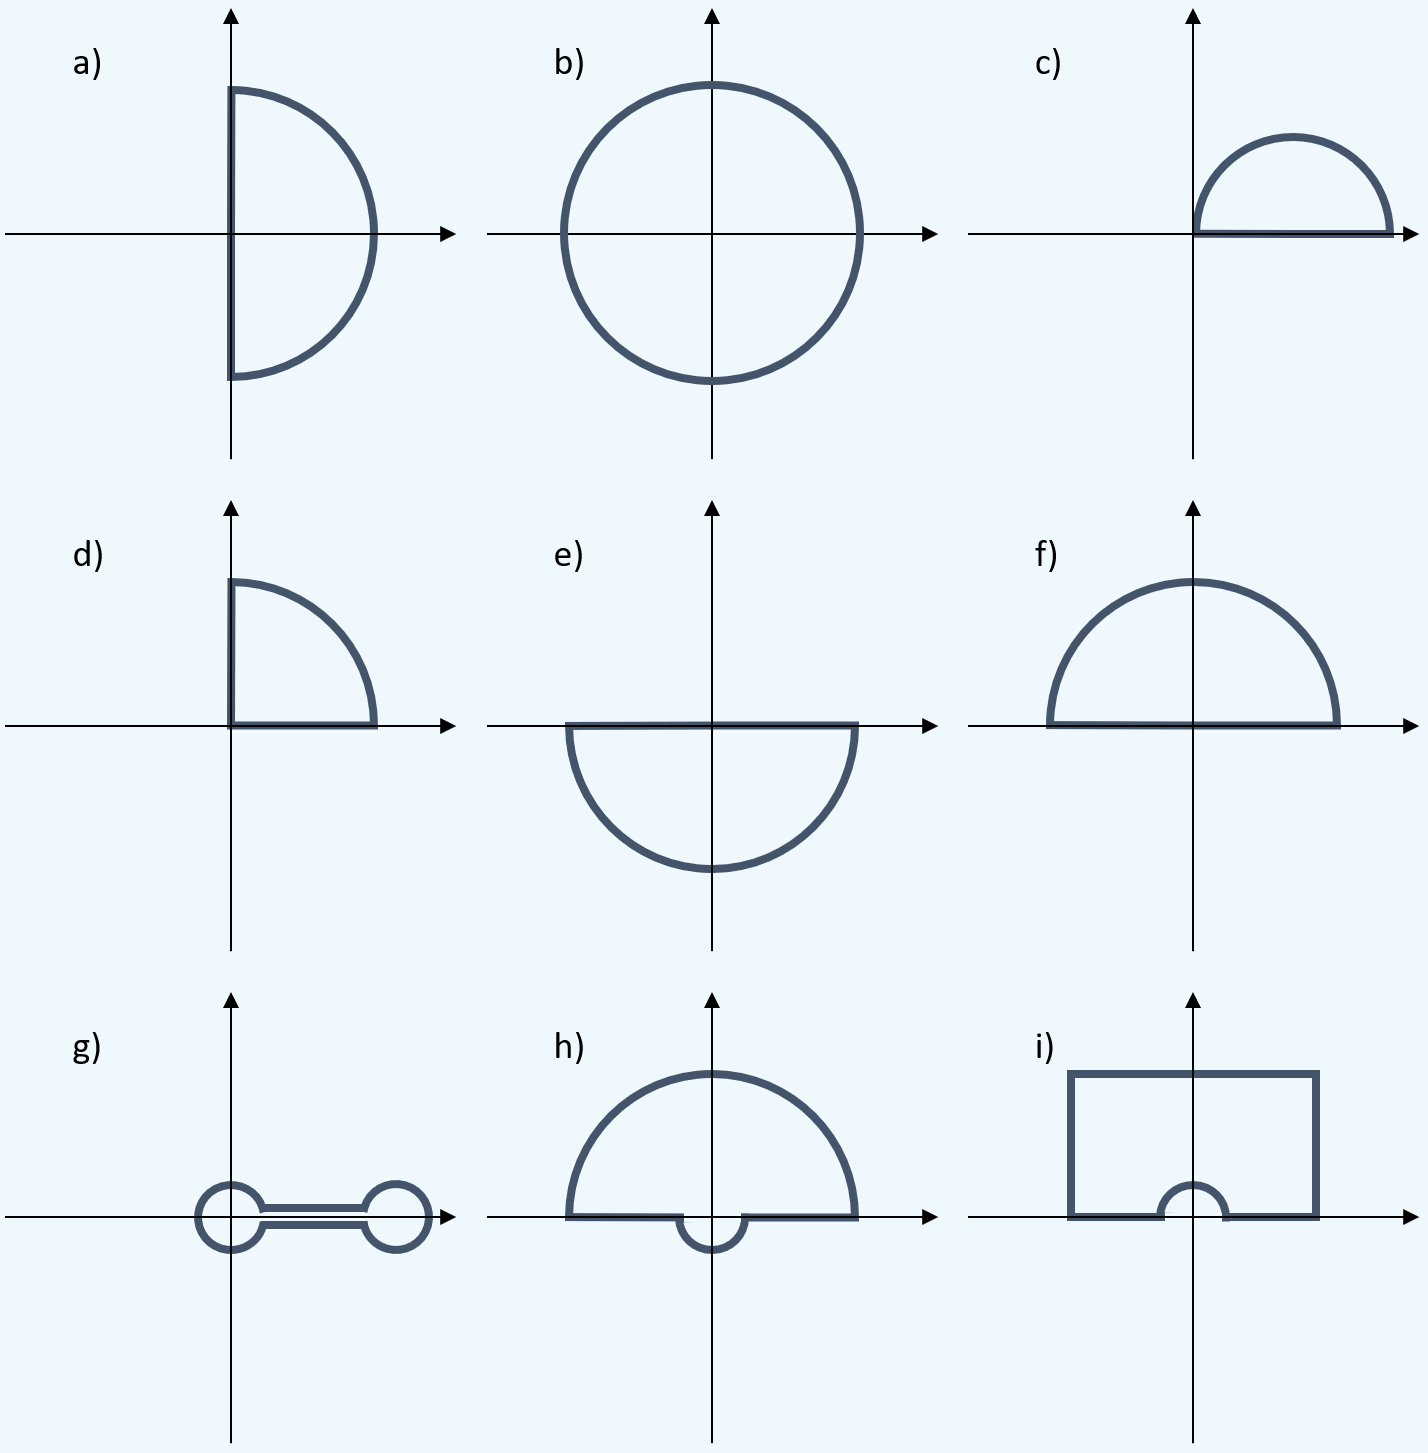
\includegraphics[width=10cm]{complex/figures/contours}
\end{center}
  
\end{exer}

\begin{exer}
% difficulty: normal
% ugent
Use complex contour integration to calculate
$$ \int_0^{\infty} \frac{\sin x}{x} dx$$
\begin{sol}
$$\frac{\pi}{2}$$
\end{sol}
\end{exer}

\pagebreak

\begin{exer}
% difficulty: normal
Use complex contour integration to calculate
$$ \int_0^{\infty} \frac{1}{\left(x^2 + a^2\right)^2} dx$$
Here $a$ is a positive real-valued number.
\begin{sol}
$$\frac{\pi}{4 a^3}$$
\end{sol}
\end{exer}

\begin{exer}
% difficulty: normal
Use complex contour integration to calculate
$$ \int_{-\infty}^{\infty} \frac{\sin \pi x}{x (x-1) (x-2)} dx$$
\begin{sol}
$$2 \pi$$
\end{sol}
\end{exer}

\begin{exer}
% difficulty: normal
Use complex contour integration to calculate
$$ \int_0^{2\pi} \frac{\cos^2 \theta d \theta}{13-5\cos 2 \theta}$$
\begin{sol}
$$\frac{\pi}{10}$$
\end{sol}
\end{exer}

\begin{exer}
% difficulty: hard
Use complex contour integration to calculate
$$ \int_0^\pi \sin^{2n} \theta d \theta$$
Here, $n \ge 1$.
\begin{sol}
$$\frac{(2n)!}{ 2^{2n}(n!)^2} \pi$$
\end{sol}
\end{exer}

\begin{exer}
% difficulty: hard
Use complex contour integration to calculate
$$ \int_0^\infty \frac{x ^ {2m}}{x^{2n} + 1} dx$$
Here $m$ and $n$ are integers and $0 \le m < n$.
\begin{sol}
$$\frac{\pi}{2n} \mathrm{cosec} \left( \frac{2m+1}{2n} \pi \right)$$
\end{sol}
\end{exer}


\pagebreak


\sectionugent{Application: Kramers--Kronig dispersion relations}

Suppose $f(z)$ is an analytic function with $\lim_\infty f(z) = 0$ in the upper half of the complex plane.

\begin{marginfigure}[-0.5cm]
\centering
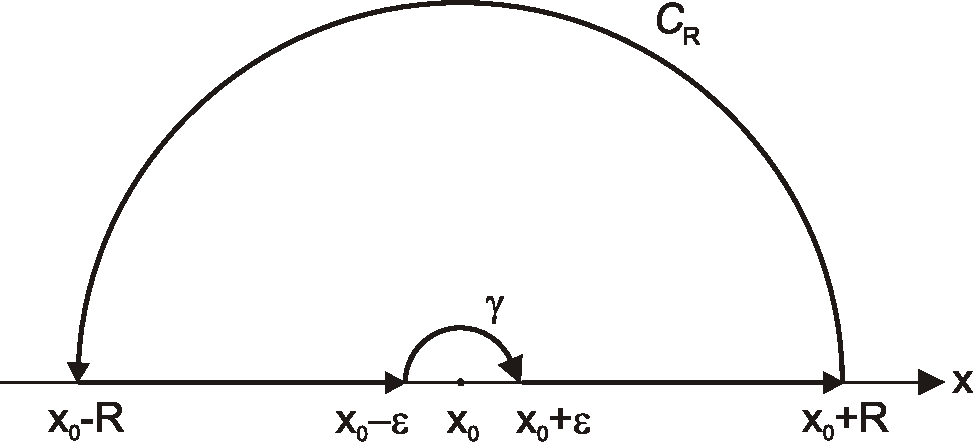
\includegraphics{complex/figures/kk}
\caption{Contour for Kramers--Kronig dispersion relations.}
\label{fig-KK}
\end{marginfigure}

Applying Cauchy's theorem to the contour in Fig.~\ref{fig-KK} leads to

\begin{equation}
\oint_{{C}} \frac{f(z)}{z-x_0} dz = 0
\end{equation}

\begin{cue}
Split up the contour integral into contributions from its different parts.
\end{cue}

\begin{marginfigure}[1.0cm]
  % credits: Wikipedia
  % url: https://en.wikipedia.org/wiki/Hans_Kramers
  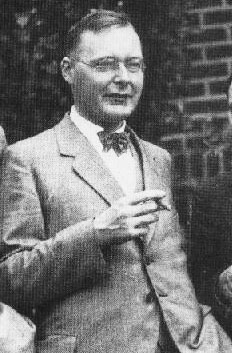
\includegraphics[]{complex/figures/h_kramers}
  \caption{Hans Kramers (1894–1952)}
\end{marginfigure}

The integral over the large semi--circle vanishes because of the big limit theorem. For the contribution of the small semi--circle around the pole $x_0$ we could use the small limit theorem, or alternatively calculate it directly:

\begin{align}
\lim_{\epsilon \to 0} & \int_{- \infty}^{x_0-\epsilon} \frac{f(x)}{x-x_0}dx + \nonumber \\
\lim_{\epsilon \to 0} & \int_{\pi}^0 \frac{f(x_0+\epsilon e^{j \theta})}{\epsilon e^{j\theta}} \epsilon j e^{j \theta} d \theta + \nonumber \\
\lim_{\epsilon \to 0} & \int_{x_0+\epsilon}^{\infty} \frac{f(x)}{x-x_0}dx = 0
\end{align} 

This leads to 

\begin{equation}
f(x_0) = \frac{1}{\pi j} PV \int_{- \infty}^{\infty} \frac{f(x)}{x-x_0}dx
\label{eq-kk-1}
\end{equation} 

If you squint a bit, you could say that the singularity $x_0$ lies more or less on our contour (although we avoided it with the small semicircle). You could therefore say that it's halfway between a singularity outside of the contour (Cauchy's theorem) and one inside the contour (Cauchy's formula). This is also reflected in the result of the integral, which is the average of these two cases, with an extra principal value thrown in for good measure.

\begin{exer}
% difficulty: trivial 
Show that Eq.~\ref{eq-kk-1} can also be obtained by choosing a contour that circles around $x_0$ in the lower half of the complex plane.
\end{exer}

\begin{cue}
Split up Eq.~\ref{eq-kk-1} into its real and imaginary parts to derive expressions for $ u(x_0)= \Re f(x_0)$ and $ v(x_0)= \Im f(x_0)$.
\end{cue}

\begin{marginfigure}[-1.5cm]
  % credits: Wikipedia
  % url: https://en.wikipedia.org/wiki/Ralph_Kronig
  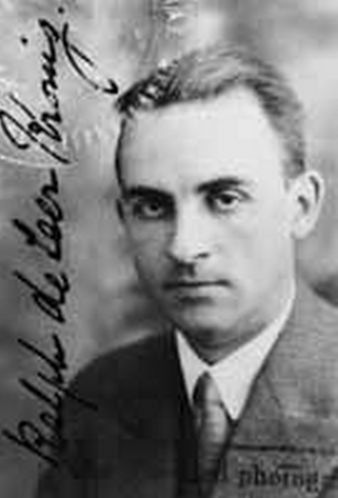
\includegraphics{complex/figures/r_kronig}
  \caption{Ralf Kronig (1904–1995)}
\end{marginfigure}

Splitting Eq.~\ref{eq-kk-1} into real and imaginary parts yields

\begin{align}
f(x_0) =& \, u(x_0) + jv(x_0) \nonumber \\
       =& \, \frac{1}{\pi j} PV \int_{- \infty}^{\infty} \frac{u(x)+jv(x)}{x-x_0}dx
 \nonumber \\
       =& \, \frac{1}{\pi} PV \int_{- \infty}^{\infty} \frac{v(x)}{x-x_0}dx -
\frac{j}{\pi} PV \int_{- \infty}^{\infty} \frac{u(x)}{x-x_0}dx
\end{align}

or

\begin{subequations} 
\begin{equation}
u(x_0) = \frac{1}{\pi} PV \int_{- \infty}^{\infty} \frac{v(x)}{x-x_0}dx
\end{equation} 
\begin{equation}
v(x_0) = -\frac{1}{\pi} PV \int_{- \infty}^{\infty} \frac{u(x)}{x-x_0}dx
\end{equation}
\label{eq-KK}
\end{subequations}

\begin{marginfigure}[-1.5cm]
  % credits: Wikipedia
  % url: https://en.wikipedia.org/wiki/David_Hilbert
  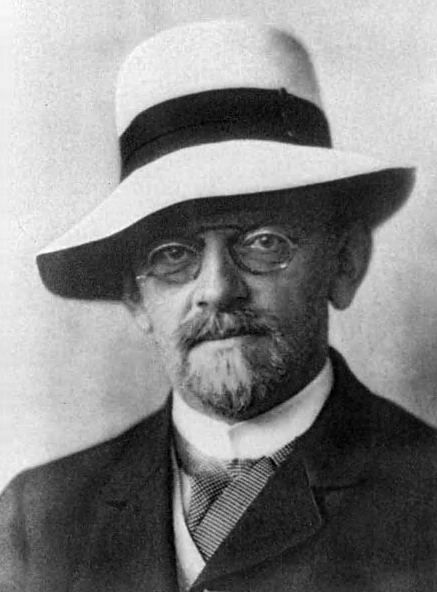
\includegraphics{complex/figures/d_hilbert}
  \caption{David Hilbert (1862–1943)}
\end{marginfigure}

Equations \ref{eq-KK} are called the \emph{Kramers--Kronig} dispersion relations. They state that under the conditions given above, the real part of a function can be expressed as an integral over the imaginary part and vice--versa.

By definition, equations \ref{eq-KK} also express that the real and imaginary parts are \emph{Hilbert transforms} of each other. Hilbert transforms also find use in e.g. telecommunications.

Let's now apply this to the field of material dispersion by applying these relations to the function $f(z) = \chi(\omega) =
n(\omega)^2 -1$. $\chi(\omega)$ is a material's susceptibility and relates the polarisation $\mathbf{P}$ to the incident electric field $\mathbf{E}$ according to $\mathbf{P}(\omega)=\varepsilon_0 \chi(\omega) \mathbf{E}(\omega)$).

\begin{exer}
% difficulty: normal
What is the mathematical reason we used $f(z) = \chi(\omega)$ here, and not e.g. $f(z) = n(\omega)$? Link this to the physics of the problem. 
\end{exer}

Replacing $x_0$ by $\omega$, and $x$ by $\omega'$, we get

\begin{subequations} 
\begin{equation}
\Re \chi(\omega) = \frac{1}{\pi} PV \int_{- \infty}^{\infty} \frac{\Im
\chi(\omega')}{\omega'-\omega}d\omega'
\end{equation} 
\begin{equation}
\Im \chi(\omega) = -\frac{1}{\pi} PV \int_{- \infty}^{\infty} \frac{\Re
\chi(\omega')}{\omega'-\omega}d\omega'
\end{equation}
\label{eq-KK-2}
\end{subequations}

As you might remember, the imaginary part of the refractive index $n$ is a measure for optical absorption. So, this means e.g. that in theory it is enough to measure the losses of a material over a wide wavelength range to calculate its refractive index.

\begin{exer}
  % difficulty: normal
Suppose you have a material without dispersion, i.e. where the real part of the squared refractive index is constant. Show that such a material is lossless, i.e. the imaginary part of the squared refractive index is zero.
\end{exer}

\begin{exer}
  % difficulty: trivial
From basic logic and the result above, conclude that as soon as you have loss in a material, the material is necessarily dispersive. Also, convince yourself that the only non-dispersive material is vacuum.
\end{exer}

Recall the definition of the susceptibility in the time domain:

\begin{equation}
\mathbf{P}(t)=\varepsilon_0 \int_{-\infty}^t \chi(t-t') \mathbf{E}(t')\, dt'.
\end{equation}

From this, we can easily see that $\chi(t)$ is necessarily real, as complex numbers only show up in the frequency domain after the introduction of phasors. From this, one can derive that for its Fourier transform $\chi(-\omega) = \chi^*(\omega)$, which in turn has some implications on the even and odd character of the real and the imaginary parts of $\chi(\omega)$. These can be used to reformulate the Kramers--Kronig relations in another common form:

\begin{exer}
  % difficulty: normal
Given that $\chi(t)$ is real-valued, show that the Kramers--Kronig dispersion relations reduce to
$$\Re \chi(\omega) =  \frac{2}{\pi} PV \int_{0}^{\infty}{ \frac{\omega'\Im \chi(\omega')}{\omega'^2-\omega^2}d\omega'}$$
$$\Im \chi(\omega) = -\frac{2}{\pi} PV \int_{0}^{\infty}{ \frac{\omega \Re \chi(\omega')}{\omega'^2-\omega^2}d\omega'}$$
\end{exer}

Finally, it's important to note that one can prove that there is a relation between the Kramers--Kronig dispersion relations and the fact that the systems considered are \emph{causal} (i.e. effect cannot precede cause)\noindent\marginnote{This is one of the subjects of the Titchmarsh theorem.}. Thus, there is an immediate physical significance of the Kramers--Kronig dispersion relations.


\pagebreak


\sectionugent{Conformal transformations}

\subsection*{Angle--preserving transformations}

\begin{marginfigure}
\centering
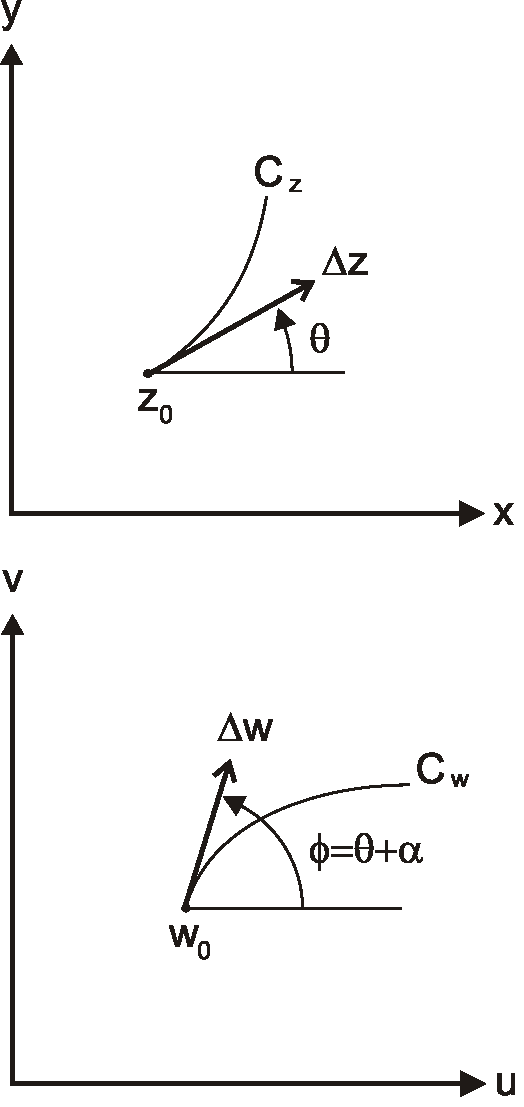
\includegraphics{complex/figures/conformal_portrait}
\caption{Conformal transformation.}
\label{fig-conformal}
\end{marginfigure}

A complex function $w = f(z) = u(x,y)+jv(x,y)$ can be seen as a mapping from the complex $z$--plane to the complex $w$--plane. One way to visualise this is to plot how a curve $C_z$ in the $z$--plane is transformed to a curve $C_w$ in the $w$--plane (see Fig.~\ref{fig-conformal}).

We can play this transformation game using two specific neighbouring points on $C_z$, e.g. $z_0$ and $z_0+\Delta z$. They get transformed to two neighbouring points on $C_w$, which we'll call imaginatively $w_0$ and $w_0+\Delta w$. In the limit of $\Delta z \to 0$, this will allow us to same something about the relationship between the tangents at the points $z_0$ and $w_0$.

\begin{cue}
Relate $\frac{df}{dz}$ to $\Delta z$ and $\Delta w$. Then look at the angles of the resulting expression to determine how the tangents rotate.
\end{cue}

As long as $w=f(z)$ is an analytic function, we have

\begin{equation}
\frac{df}{dz} = \frac{dw}{dz} = \lim_{\Delta z \to 0} \frac{\Delta w}{\Delta z}
\end{equation}

By putting this expression in polar form and looking at the angle, we can derive an expression relating the angles of the tangents at $z_0$ and $w_0$:

\begin{equation}
\arg \frac{df}{dz} = \arg \lim_{\Delta z \to 0} \frac{\Delta w}{\Delta z} = \arg
\lim_{\Delta z   \to 0} \Delta w - \arg \lim_{\Delta z \to 0} \Delta z
\end{equation} 

For an analytic function $\arg df / dz = \alpha$ (the angle of the derivative) depends on $z$, but for a given $z$ it is independent of the direction of approach. So, if in Fig.~\ref{fig-conformal} the angle of the increment $\Delta z$ with respect to the $x$--axis is $\theta$, and the increment $\Delta w$ forms an angle $\phi$ with the $u$ axis, we can relate these angles by

\begin{equation}
\phi = \theta + \alpha
\end{equation}

This also means that an analytic transformation will rotate any line in the $z$--plane over an angle of $\alpha$ in the $w$--plane. Since this result holds for any line through $z_0$, it obviously also holds for any \emph{pair} of lines. This means that for the angle between these two lines we get

\begin{equation}
\phi_2 - \phi_1 = (\theta_2 + \alpha) - (\theta_1 + \alpha) = \theta_2 -
\theta_1
\end{equation} 

From this we can see that such a transformation preserves the angle between any pair of lines. If such an angle--preserving transformation defined by an analytic function is also injective between two domains, it is called a \emph{conformal transformation}.

\subsection*{Conformal transformations and the Helmholtz equation}

Conformal transformations can be useful to solve the Helmholtz equation in a 'difficult' coordinate system. The idea is to use a conformal mapping to transform the coordinate system to a different one where the solution is more tractable. In this section, we will investigate what form the Helmholtz equation takes in the new domain.

Suppose our old $(x,y)$--coordinate system is related to a new $(u,v)$--coordinate system by a conformal transformation $f$:

\begin{equation}
u+jv = w = f(z) = f(x+jy)
\end{equation} 

In the $z$--plane, the Helmholtz equation in media with piecewise constant refractive index has the following form:

\begin{equation}
\frac{\partial^2 \psi(x,y)}{\partial x^2} + \frac{\partial^2 \psi(x,y)}{\partial y^2} + k_0^2 n^2(x,y) \psi(x,y) = 0
\end{equation}

\begin{cue}
Use the chain rule to express $\frac{\partial \psi}{\partial x}$ using partial derivatives with respect to $u$ and $v$.
\end{cue}

Application of the chain rule leads to

\begin{equation}
\frac{\partial \psi}{\partial x} = \frac{\partial \psi}{\partial u}
\frac{\partial u}{\partial x} + \frac{\partial \psi}{\partial v} \frac{\partial
v}{\partial x}
\end{equation} 

\begin{cue}
Now calculate $\frac{\partial^2 \psi}{\partial x^2}$.
\end{cue}

For the second derivative this becomes

\begin{equation}
\frac{\partial^2 \psi}{\partial x^2} = \frac{\partial}{\partial x} \left[
\frac{\partial \psi}{\partial u}\right]  \frac{\partial u}{\partial x} +
\frac{\partial \psi}{\partial u}\frac{\partial^2 u}{\partial x^2} +  
\frac{\partial}{\partial x} \left[ \frac{\partial \psi}{\partial v}\right] 
\frac{\partial v}{\partial x}  + \frac{\partial \psi}{\partial
v}\frac{\partial^2 v}{\partial x^2}
\end{equation} 

Or

\begin{align}
\frac{\partial^2 \psi}{\partial x^2} = &\left[ \frac{\partial^2 \psi}{\partial u^2 } \frac{\partial u}{\partial x} +  \frac{\partial^2 \psi}{\partial u \partial v} \frac{\partial v}{\partial x} \right] \frac{\partial u}{\partial x}  + \frac{\partial \psi}{\partial u}\frac{\partial^2 u}{\partial x^2} \nonumber \\ 
+ &\left[ \frac{\partial^2 \psi}{\partial v^2 } \frac{\partial v}{\partial x} + 
\frac{\partial^2 \psi}{\partial u \partial v} \frac{\partial u}{\partial x}
\right] \frac{\partial v}{\partial x} + \frac{\partial \psi}{\partial v}\frac{\partial^2 v}{\partial x^2}
\end{align} 

\begin{cue}
Now add these two second-order derivatives and go on a term-cancelling spree. Remember that the Cauchy-Riemann conditions hold. Also, note that for a holomorphic function $\nabla^2 u = \nabla^2 v=0$.
\end{cue}

For the total Laplacian we get

\begin{align}
\frac{\partial^2 \psi}{\partial x^2} &+ \frac{\partial^2 \psi}{\partial y^2}= \nonumber \\
  &\frac{\partial^2 \psi}{\partial u^2 }  \left [ \left(\frac{\partial u}{\partial x}\right)^2 + \left(\frac{\partial u}{\partial y}\right)^2\right]+ \frac{\partial \psi}{\partial u} \left[ \frac{\partial^2 u}{\partial x^2}  + \frac{\partial^2 u}{\partial y^2} \right] + 2\frac{\partial^2 \psi}{\partial u \partial v} \frac{\partial u}{\partial x} \frac{\partial v}{\partial x}    \nonumber \\  
+ &\frac{\partial^2 \psi}{\partial v^2}  \left[ \left(\frac{\partial v}{\partial
x}\right)^2 + \left(\frac{\partial v}{\partial y}\right)^2\right] + \frac{\partial
\psi}{\partial v} \left[ \frac{\partial^2 v}{\partial x^2} + \frac{\partial^2 v}{\partial y^2} \right] + 2\frac{\partial^2 \psi}{\partial u \partial v} \frac{\partial u}{\partial y} \frac{\partial v}{\partial y}
\label{eq-conf-trans-1}
\end{align} 

It is easy to see that terms three and six cancel because of the Cauchy--Riemann conditions.

We know from Ex.~\ref{ex-harmonic} that for a holomorphic function $\nabla^2 u =
\nabla^2 v=0$, so the second and the fifth term on the right--hand--side of
Eq.~\ref{eq-conf-trans-1} vanish as well.

\begin{cue}
What does Cauchy--Riemann teach us about the factors in square brackets in terms one and four?
\end{cue}

Because of the Cauchy--Riemann equations, we can write

\begin{equation}
\left(\frac{\partial u}{\partial x}\right)^2 + \left(\frac{\partial u}{\partial
y}\right)^2 = \left(\frac{\partial v}{\partial x}\right)^2  +
\left(\frac{\partial v}{\partial y}\right)^2 = 
\left(\frac{\partial u}{\partial x}\right)^2 + \left(\frac{\partial v}{\partial
x}\right)^2 
 \stackrel{def}{=} \frac{1}{T(u,v)^2} \label{eq-T-factor}
\end{equation} 

So finally, we can write the Helmholtz equation in the transformed domain as

\begin{equation}
\frac{\partial^2 \psi(u,v)}{\partial u^2} + \frac{\partial^2 \psi(u,v)}{\partial
v^2} + k_0^2 T^2(u,v)n^2(u,v) \psi(u,v) = 0
\end{equation} 

Formally, this is identical to the Helmholtz equation in the $z$--plane, except that \emph{the index distribution $n$ has been replaced by a transformed index distribution $T \cdot n$}.

\subsection*{Application: bent waveguides}

\begin{marginfigure}[-6cm]
\centering
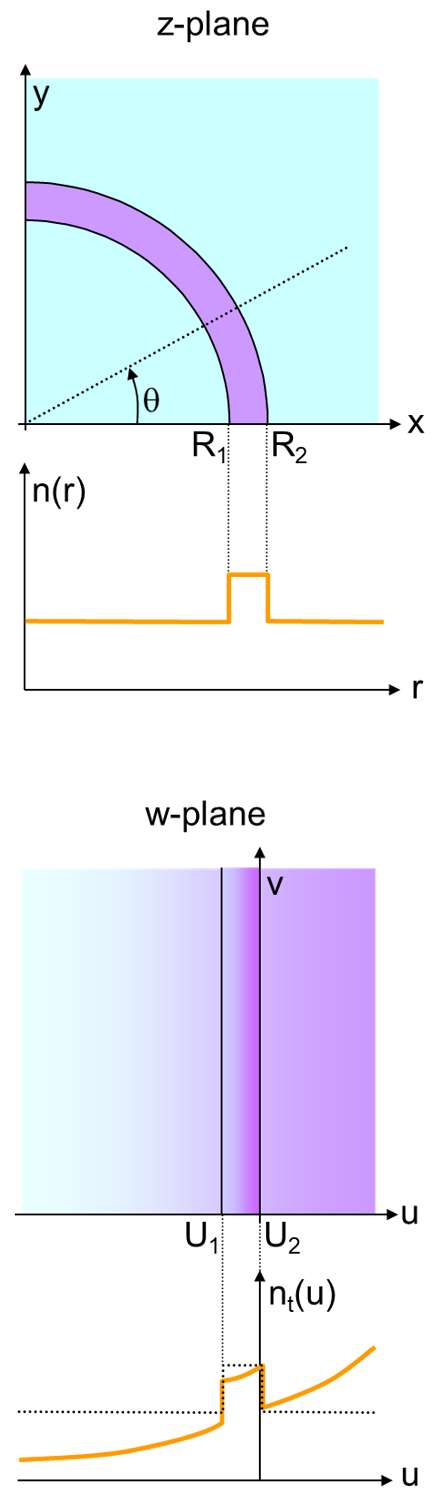
\includegraphics{complex/figures/bends_portrait}
\caption{Calculating bend modes using conformal transformation.}
\label{fig-bends}
\end{marginfigure}

To give an example of the power of conformal transformations, we will use it to find the eigenmodes of a bent dielectric waveguide (Fig.~\ref{fig-bends}). We consider the system to be invariant in the $z$--direction.

To tackle this problem, we could formulate the Helmholtz equation in cylindrical
coordinates, and the solution would involve Bessel functions. Here however, we will use the following conformal transformation to convert the curved geometry to a straight one:

\begin{equation}
w = R_2 \ln \frac{z}{R_2}
\end{equation} 

\begin{cue}
Transform this to polar coordinates and verify that this indeed straightens the bend.  
\end{cue}

With $z=r e^{j \theta}$, we can write this as

\begin{equation}
u + jv = R_2 \ln \frac{r}{R_2} + j R_2 \theta
\end{equation} 

This clearly shows the effect of the transformation: a circular path in the $z$--plane with constant $r$ is transformed to a straight path in the $w$--plane with constant $u$ (see Fig.~\ref{fig-bends}).

\begin{cue}
Calculate the transformation factor $T$. 
\end{cue}

Using the definition of the transformation factor $T$ from Eq.~\ref{eq-T-factor}, we get

\begin{equation}
\frac{\partial u}{\partial x} = \frac{R_2}{r}\frac{\partial r}{\partial x} = 
\frac{R_2}{\sqrt{x^2+y^2}} \cdot \frac{2x}{2\sqrt{x^2+y^2}} = R_2
\frac{x}{x^2+y^2}
\end{equation} 

Also,

\begin{equation}
\frac{\partial v}{\partial x} = R_2 \frac{\partial}{\partial x} \arctan
\frac{y}{x} = \frac{R_2}{1 + \frac{y^2}{x^2}} \cdot y \cdot \frac{-1}{x^2}= -R_2
\frac{y}{x^2+y^2}
\end{equation} 

So finally

\begin{equation}
T = \frac{1}{\sqrt{u_x^2+v_x^2}} = \frac{\sqrt{x^2+y^2}}{R_2} =
\frac{r}{R_2}=e^{\frac{u}{R_2}}
\end{equation} 

In the new coordinate system, the transformed index profile looks like

\begin{equation}
n_t(u) = n(u)e^{\frac{u}{R_2}}
\end{equation} 

This profile is sketched in Fig.~\ref{fig-bends}. The rest of the solution now proceeds as follows. The continuous index profile is approximated by a stepwise constant profile with a large number of steps. The modes of such a waveguide can be readily found by using standard techniques.

When this way of calculating the modes of a bent waveguide was first proposed in the 1970s, the calculation power of computers was nothing to write home about, so any trick that could simplify a problem was very welcome. Today, the interest of these techniques is more instructional than practical, although it does allow us to get some physical insight.

\begin{cue}
Making use of the tendency of light to concentrate in regions with high refractive index, think about how light in these bent waveguides will behave. What happens if the radius of curvature decreases?  
\end{cue}

Because the refractive index is higher near the outside of the bend, the mode will tend to be concentrated there. There is also the opportunity for the light to tunnel towards the outer cladding, where the index is even higher. This is the origin of the radiation losses in waveguide bends. Tighter bends (i.e. shorter radii) will be more prone to this phenomenon, because the steeper exponential will reduce the tunneling distance.


\section*{Review questions}

\begin{itemize}
\item What is a holomorphic function?
\item What are the Cauchy-Riemann conditions?
\item What is Cauchy's theorem?
\item What is Cauchy's formula?
\item What is a Laurent series?
\item What type of poles can a function have?
\item What are branch points and branch cuts?
\item What is the Riemann surface?
\item What is a residue?
\item How do you calculate the residue of a single pole?
\item What is the residue theorem?
\item What is Jordan's lemma?
\item What are the big and small limit theorems?
\item What is the principal value of an integral?
\item How do you solve integrals of the type $\int_0^{2 \pi} f(\cos \theta, \sin \theta) d \theta$?
\item How do you solve integrals of the type  $\int_\infty^{\infty} f(z) e^{jbz} dz$?
\item What do the Kramers-Kronig relations express?
\item What are conformal transformations and what are they used for?
\end{itemize}

%%% Local Variables:
%%% mode: latex
%%% TeX-master: "../main"
%%% End:
